\newpage
\chapter{METODE PENELITIAN} \label{BabIII}
\section{Alur Penelitian} \label{III.Alur}
Alur penelitian pada tugas akhir ini disajikan dalam bentuk flowchart untuk memvisualisasikan tahapan secara sistematis, mulai dari perencanaan, pengumpulan data, pra-pemrosesan, pelatihan model, hingga evaluasi. Fokus penelitian ini adalah pengenalan gerakan Sistem Isyarat Bahasa Indonesia (SIBI) berbasis citra video dengan menggunakan arsitektur Video Masked Autoencoder (VideoMAE) sebagai model utama dalam proses ekstraksi dan klasifikasi gerakan visual.\par
\begin{figure}[htbp]
\centering
\fbox{%
\resizebox{0.90\textwidth}{!}{%
\begin{tikzpicture}[scale=0.7,
  node distance = 5mm and 5mm,
  startstop/.style = {rectangle, rounded corners=10pt,
    minimum width=28mm, minimum height=9mm, align=center,
    font=\small, draw=black, line width=0.6pt, fill=white},
  process/.style  = {rectangle, rounded corners=3pt,
    minimum width=28mm, minimum height=9mm, align=center,
    font=\small, draw=black, line width=0.5pt, fill=white},
  arr/.style = {-{Stealth[length=4pt]}, line width=0.6pt, black}
]
  % Baris 1: kiri → kanan
  \node[startstop]               (start) {Mulai};
  \node[process, right=of start] (n1)    {Identifikasi\\Masalah};
  \node[process, right=of n1]    (n2)    {Studi Literatur};
  % Baris 2: kanan → kiri
  \node[process, below=of n2]    (n3)    {Pengumpulan\\Data};
  \node[process, left=of n3]     (n4)    {Pra-pemrosesan\\Data};
  \node[process, left=of n4]     (n5)    {Pelatihan Model};
  % Baris 3: kiri → kanan
  \node[process, below=of n5]    (n6)    {Evaluasi Model};
  \node[process, right=of n6]    (n7)    {Hasil dan\\Pembahasan};
  \node[startstop, right=of n7]  (end)   {Selesai};
  % Panah baris 1
  \draw[arr] (start) -- (n1);
  \draw[arr] (n1)    -- (n2);
  % Penghubung baris 1→2
  \draw[arr] (n2.south) -- (n3.north);
  % Panah baris 2
  \draw[arr] (n3) -- (n4);
  \draw[arr] (n4) -- (n5);
  % Penghubung baris 2→3
  \draw[arr] (n5.south) -- (n6.north);
  % Panah baris 3
  \draw[arr] (n6) -- (n7);
  \draw[arr] (n7) -- (end);
\end{tikzpicture}%
}%
}
\caption{Alur Penelitian}
\label{fig:3.alur}
\end{figure}
\section{Penjabaran Langkah Penelitian} \label{III.Jabar_Alur}
Bagian ini menjelaskan tahapan detail dari proses penelitian berdasarkan alur yang telah ditampilkan pada Gambar~\ref{fig:3.alur}. Setiap tahapan dilakukan secara berurutan untuk memastikan hasil akhir model klasifikasi visual yang akurat dan konsisten.\par

\subsection{Identifikasi Masalah} \label{III.Identifikasi_Masalah}
Tahap identifikasi masalah dilakukan untuk memastikan fokus penelitian disusun berdasarkan kebutuhan nyata dan memiliki dasar empiris yang jelas. Proses ini dilakukan secara sistematis melalui serangkaian langkah yang membantu peneliti menemukan permasalahan utama serta menentukan ruang lingkup penelitian yang akan dikaji. Kegiatan diawali dengan observasi awal terhadap isu komunikasi antara penyandang tunarungu dan masyarakat umum untuk memahami kondisi aktual yang terjadi di lapangan. Observasi dilakukan dengan meninjau penggunaan Bahasa Isyarat SIBI di lingkungan pendidikan dan sosial, serta menelaah tantangan yang dihadapi pengguna dalam berinteraksi tanpa penerjemah.\par

Setelah itu dilakukan penelusuran dokumen dan sumber ilmiah untuk melihat perkembangan penelitian di bidang pengenalan bahasa isyarat. Langkah ini mencakup pengumpulan jurnal, prosiding, dan laporan penelitian yang relevan dengan topik sistem pengenalan isyarat berbasis visi komputer dan pembelajaran mendalam. Setiap referensi dianalisis untuk mengidentifikasi pendekatan, algoritma, dan hasil yang telah dicapai, sekaligus menelusuri keterbatasan atau celah penelitian yang masih belum terselesaikan. Tahap berikutnya adalah analisis perbandingan hasil penelitian terdahulu dengan kebutuhan aktual di lapangan. Perbandingan ini digunakan untuk menentukan aspek teknis yang perlu dikembangkan, misalnya efisiensi model, kemampuan mengenali gerakan kompleks, serta ketahanan terhadap variasi kondisi pencahayaan dan latar.\par

Hasil dari seluruh proses tersebut menghasilkan rumusan masalah yang menjadi dasar arah penelitian ini, yaitu perlunya sistem pengenalan gerakan SIBI berbasis video yang mampu menangkap hubungan spasial dan temporal secara otomatis, mengingat belum tersedianya sistem pengenalan SIBI berbasis video yang memadai untuk mendukung komunikasi antara penyandang tunarungu dan masyarakat umum di Indonesia.\par

\subsection{Studi Literatur} \label{III.Studi_Literatur}
Tahap studi literatur dilakukan untuk memperoleh dasar teori dan referensi ilmiah yang relevan dengan fokus penelitian, yaitu pengenalan gerakan Bahasa Isyarat SIBI berbasis video. Proses ini dilakukan secara sistematis agar informasi yang dikumpulkan dapat dipertanggungjawabkan secara ilmiah dan mendukung penyusunan metode penelitian.\par

Langkah pertama yang dilakukan adalah menentukan topik dan kata kunci pencarian yang sesuai dengan ruang lingkup penelitian. Kata kunci yang digunakan meliputi istilah seperti ``pengenalan bahasa isyarat berbasis video', ``SIBI recognition', ``Video Transformer', ``VideoMAE', dan ``spatio-temporal learning'. Penentuan kata kunci ini bertujuan untuk memfokuskan pencarian pada penelitian yang relevan dan memiliki keterkaitan langsung dengan sistem pengenalan bahasa isyarat.\par

Setelah kata kunci ditetapkan, pencarian referensi dilakukan melalui basis data ilmiah seperti IEEE Xplore, SpringerLink, ScienceDirect, dan Google Scholar. Setiap referensi yang digunakan dipilih berdasarkan kriteria kredibilitas, relevansi dengan bidang computer vision, serta kesesuaian dengan topik penelitian yang sedang dikembangkan. Literatur yang dipilih mengutamakan hasil penelitian terkini dari jurnal atau prosiding yang telah ditinjau sejawat (peer-reviewed).\par

Seluruh referensi yang diperoleh kemudian dibaca dan dianalisis untuk memahami konteks penelitian terdahulu, meliputi pendekatan yang digunakan, metode pelatihan, serta hasil yang dicapai. Analisis dilakukan secara deskriptif dengan menyoroti kelebihan dan keterbatasan dari setiap pendekatan tanpa melakukan pengelompokan formal atau klasifikasi tematik. Hasil analisis ini digunakan untuk mengidentifikasi celah penelitian yang masih ada dan menentukan arah pengembangan metode yang sesuai.\par

Tahap akhir dari studi literatur adalah penyusunan ringkasan hasil kajian dalam bentuk narasi dan tabel literasi penelitian terdahulu yang berisi nama peneliti, tahun, metode yang digunakan, serta hasil utama dari penelitian. Melalui tahapan ini, peneliti memperoleh dasar teoritis dan teknis yang kuat untuk mendukung penerapan arsitektur VideoMAE dalam sistem pengenalan gerakan Bahasa Isyarat SIBI berbasis video.\par

\subsection{Pengumpulan Data} \label{III.Pengumpulan_Data}
Tahap pengumpulan data dilakukan untuk memperoleh dataset yang akan digunakan dalam proses pelatihan dan pengujian sistem penerjemah bahasa isyarat. Data yang dikumpulkan berupa video gerakan tangan dan ekspresi wajah dari pengguna Sistem Isyarat Bahasa Indonesia (SIBI) yang mewakili kata-kata dasar.\par
Pengambilan dataset dilakukan secara langsung di Sekolah Luar Biasa Negeri (SLBN) PKK Provinsi Lampung dengan melibatkan peserta didik dan guru pendamping yang fasih berkomunikasi menggunakan SIBI. Setiap pengambilan sampel diawali dengan pengarahan mengenai daftar kosakata, prosedur perekaman, serta protokol etika agar peserta merasa nyaman saat berada di depan kamera. Proses perekaman dilakukan dalam ruangan tertutup dengan pencahayaan stabil, latar belakang polos, dan tingkat kebisingan rendah sehingga kualitas video seragam dan bebas gangguan visual.\par
Video direkam menggunakan kamera digital beresolusi minimal 1080p pada 30 fps yang dipasang pada tripod setinggi bahu peserta. Jarak kamera dijaga pada rentang 1{,}5--2 meter agar area gerak visual terekam dengan jelas. Setiap isyarat direkam dalam beberapa ulangan untuk mengantisipasi kesalahan gerak atau variasi antarpenutur. Dataset yang dihasilkan terdiri dari 10 kata dasar yang sering digunakan dalam lingkungan sekolah (aku, kamu, suka, sekolah, pulang, mau, bawa, ibu, bapak, guru). Setiap isyarat direkam beberapa kali untuk memastikan variasi gerakan dan konsistensi data. Setelah proses perekaman selesai, seluruh data dikonversi ke format seragam (MP4) dan diberi label teks padanan Bahasa Indonesia. Pembagian dataset menggunakan skema \textit{Stratified 5-Fold Cross Validation} dengan rasio 80:20 (\textit{train}:\textit{validation}) pada setiap fold, sehingga setiap klip memperoleh kesempatan menjadi data validasi tepat satu kali tanpa adanya subset uji terpisah.\par
Skema pengambilan data ditunjukkan pada Gambar~\ref{fig:3.skemadatapengumpulan}. 
Skema ini menggambarkan tahapan sistematis dari proses perekaman hingga penyimpanan data 
yang siap digunakan pada tahap pra-pemrosesan.\par
\begin{figure}[H]
\centering
\fbox{%
\resizebox{0.90\textwidth}{!}{%
\begin{tikzpicture}[scale=0.7,
  node distance = 5mm and 5mm,
  startstop/.style = {rectangle, rounded corners=10pt,
    minimum width=28mm, minimum height=9mm, align=center,
    font=\small, draw=black, line width=0.6pt, fill=white},
  process/.style  = {rectangle, rounded corners=3pt,
    minimum width=28mm, minimum height=9mm, align=center,
    font=\small, draw=black, line width=0.5pt, fill=white},
  decision/.style = {diamond, aspect=1.6,
    minimum width=28mm, align=center,
    font=\small, draw=black, line width=0.5pt, fill=white},
  arr/.style = {-{Stealth[length=4pt]}, line width=0.6pt, black}
]
  % Baris 1: kiri → kanan
  \node[startstop]               (start) {Mulai};
  \node[process, right=of start] (n1)    {Pemilihan\\Responden};
  \node[process, right=of n1]    (n2)    {Perekaman\\Gerakan SIBI};
  \node[decision, right=of n2]   (dec)   {Data\\Valid?};
  % Baris 2: kanan → kiri
  \node[process,  below=of dec]  (n3)    {Konversi Format\\(MP4)};
  \node[process,  left=of n3]    (n4)    {Pemberian\\Label Data};
  \node[process,  left=of n4]    (n5)    {Penyimpanan\\Dataset};
  \node[startstop,left=of n5]    (end)   {Selesai};
  % Panah baris 1
  \draw[arr] (start) -- (n1);
  \draw[arr] (n1)    -- (n2);
  \draw[arr] (n2)    -- (dec);
  % Baris 1→2: Ya
  \draw[arr] (dec.south) -- node[right,font=\scriptsize]{Ya} (n3.north);
  % Panah baris 2
  \draw[arr] (n3) -- (n4);
  \draw[arr] (n4) -- (n5);
  \draw[arr] (n5) -- (end);
  % Loop Tidak: naik, lalu kiri ke n2
  \draw[arr] (dec.north) -- ++(0,7mm) --
    node[above,font=\scriptsize]{Tidak} ($(n2.north)+(0,7mm)$) -- (n2.north);
\end{tikzpicture}%
}%
}
\caption{Skema Pengumpulan Data}
\label{fig:3.skemadatapengumpulan}
\end{figure}
\noindent
Skema pada Gambar~\ref{fig:3.skemadatapengumpulan} menggambarkan alur proses pengambilan data 
yang dilakukan di SLBN PKK Provinsi Lampung. Proses dimulai dari tahap \textit{Start} yang menandai 
awal kegiatan pengumpulan data. Tahap pertama adalah pemilihan responden, yaitu menentukan guru 
atau siswa yang memiliki kemampuan berkomunikasi menggunakan SIBI sebagai subjek penelitian. 
Selanjutnya dilakukan perekaman gerakan SIBI, di mana setiap responden menampilkan gerakan tangan, 
ekspresi wajah, serta posisi tubuh yang sesuai. Hasil rekaman kemudian melalui tahap validasi data 
awal untuk memastikan kualitas video sesuai standar. Jika data dinilai tidak valid, proses perekaman 
diulangi sampai diperoleh hasil yang layak digunakan.\par
Apabila data telah dinyatakan valid, langkah berikutnya adalah konversi format. Setelah itu dilakukan pemberian label data, yaitu menentukan teks Bahasa Indonesia yang sesuai dengan makna setiap gerakan isyarat. Tahap terakhir adalah penyimpanan dataset terstruktur ke dalam direktori yang diorganisasikan per kelas kata. Setiap folder diberi nama sesuai kata SIBI yang direkam dan berisi seluruh klip dengan penamaan berformat \texttt{NamaKelas\_NNN.mp4} (mis.\ \texttt{Aku\_001.mp4}), untuk memudahkan pelacakan dan pra-pemrosesan.\par Proses ini diakhiri dengan tahap \textit{End}, yang menandakan bahwa dataset siap digunakan pada tahap pra-pemrosesan dan pelatihan model.\par
\begin{lstlisting}[language=, caption={Struktur Direktori Dataset SIBI}, label={lst:struktur-dataset-visual}, numbers=none, frame=single, basicstyle=\ttfamily\small, columns=fullflexible]
Dataset/
|-- Aku/        (90 file)
|   |-- Aku_001.mp4
|   |-- Aku_002.mp4
|   `-- ...
|-- Bapak/      (90 file)
|-- Bawa/       (88 file)
|-- Guru/       (90 file)
|-- Ibu/        (96 file)
|-- Kamu/       (93 file)
|-- Mau/        (99 file)
|-- Pulang/     (100 file)
|-- Sekolah/    (89 file)
`-- Suka/       (90 file)
\end{lstlisting}


\subsection{Data Preprocessing} \label{III.Data_Preprocessing}

Tahap pra-pemrosesan data menyiapkan klip video mentah agar sesuai dengan format masukan VideoMAE sekaligus menyiapkan skema pembagian data yang digunakan selama pelatihan. Format akhir yang harus dihasilkan adalah klip berdimensi tetap $(3,16,224,224)$ sebagaimana digunakan pada arsitektur VideoMAE \cite{Tong2022VideoMAE}. Alur tahapan pra-pemrosesan secara keseluruhan ditunjukkan pada Gambar~\ref{fig:3.alur_pra}, yang mencakup standardisasi spasial dan temporal, pembagian data dengan \textit{Stratified K-Fold}, augmentasi data, penyusunan komposisi fold, serta penyimpanan metadata dalam bentuk berkas CSV.\par

\begin{figure}[H]
\centering
\fbox{%
\resizebox{0.90\textwidth}{!}{%
\begin{tikzpicture}[scale=0.7,
  node distance = 5mm and 5mm,
  startstop/.style = {rectangle, rounded corners=10pt,
    minimum width=30mm, minimum height=9mm, align=center,
    font=\small, draw=black, line width=0.6pt, fill=white},
  process/.style  = {rectangle, rounded corners=3pt,
    minimum width=30mm, minimum height=9mm, align=center,
    font=\small, draw=black, line width=0.5pt, fill=white},
  arr/.style = {-{Stealth[length=4pt]}, line width=0.6pt, black}
]
  % Baris 1: kiri → kanan
  \node[startstop]               (start) {Mulai};
  \node[process, right=of start] (n1)    {Baca Dataset\\Video \& Label};
  \node[process, right=of n1]    (n2)    {Preprocessing Video\\{\scriptsize resize $224\!\times\!224$, 30 FPS}};
  \node[process, right=of n2]    (n3)    {Stratified\\K-Fold ($k{=}5$)};
  % Baris 2: kanan → kiri
  \node[process, below=of n3]    (n4)    {Augmentasi Data};
  \node[process, left=of n4]     (n5)    {Fold Composition};
  \node[process, left=of n5]     (n6)    {Simpan Metadata\\CSV};
  \node[startstop, left=of n6]   (end)   {Selesai};
  % Panah baris 1
  \draw[arr] (start) -- (n1);
  \draw[arr] (n1)    -- (n2);
  \draw[arr] (n2)    -- (n3);
  % Penghubung baris 1→2
  \draw[arr] (n3.south) -- (n4.north);
  % Panah baris 2
  \draw[arr] (n4) -- (n5);
  \draw[arr] (n5) -- (n6);
  \draw[arr] (n6) -- (end);
\end{tikzpicture}%
}%
}
\caption{Flowchart tahapan pra-pemrosesan video}
\label{fig:3.alur_pra}
\end{figure}

Tahap pertama adalah membaca seluruh berkas video pada \textit{Dataset Video Bahasa Isyarat} beserta label kelasnya. Setiap video kemudian melalui proses \textit{Preprocessing Video} berupa \textit{resize} menjadi resolusi spasial $224\times224$ piksel dan standardisasi laju cuplik menjadi 30 FPS. Resolusi $224\times224$ dipilih agar konsisten dengan ukuran masukan standar pada arsitektur Vision Transformer dan VideoMAE \cite{Tong2022VideoMAE,Dosovitskiy2021}, sedangkan standardisasi 30 FPS diperlukan agar seluruh video memiliki kecepatan temporal yang sama sehingga panjang gestur SIBI terwakili secara konsisten pada tiap klip 16 frame yang akan disampling pada tahap pelatihan.\par

Setelah seluruh video distandardisasi, data dibagi menggunakan \textit{Stratified K-Fold Cross Validation} dengan $k=5$. Skema stratifikasi memastikan distribusi kelas pada setiap fold tetap seimbang, sehingga proporsi sepuluh kelas kata SIBI tidak terdistorsi pada subset latih maupun subset validasi. Strategi \textit{k-fold} dipilih sebagai pengganti pembagian tunggal karena ukuran dataset yang relatif terbatas; dengan menjalankan lima lipatan, setiap sampel video memperoleh kesempatan menjadi data validasi tepat satu kali, sehingga estimasi performa model menjadi lebih stabil dan minim bias akibat pembagian data acak tunggal.\par

Secara paralel dengan proses pembagian fold, sistem melakukan \textit{Data Augmentation} pada data video untuk memperkaya variasi sampel latih. Tiga jenis augmentasi diterapkan, yaitu (1) \textit{inversion} berupa pembalikan horizontal frame untuk mensimulasikan perbedaan tangan dominan penutur, (2) \textit{brightness adjustment} untuk menirukan variasi pencahayaan ruangan, dan (3) \textit{downsampling} frame untuk menghasilkan variasi kecepatan gerak isyarat. Ketiga augmentasi ini dipilih karena tidak mengubah makna gestur SIBI namun mampu menghadirkan variasi yang relevan dengan kondisi dunia nyata, sehingga model dapat belajar fitur yang lebih invarian terhadap perubahan-perubahan tersebut.\par

Hasil augmentasi kemudian digabungkan dengan data asli pada tahap \textit{Fold Composition}. Pada setiap fold, subset latih disusun dari gabungan video asli dan video hasil augmentasi, sedangkan subset validasi hanya berisi video asli tanpa augmentasi. Pemisahan ini penting agar metrik validasi merepresentasikan performa model pada data yang bersih dan tidak tercampur dengan distribusi augmentasi, sehingga evaluasi antar fold tetap adil dan dapat dibandingkan. Strategi augmentasi hanya pada subset latih juga mencegah kebocoran informasi dari data augmentasi ke proses validasi.\par

Langkah terakhir pada tahap pra-pemrosesan adalah menyimpan metadata setiap video ke dalam berkas CSV. Berkas ini mencatat path video, label kelas, indeks fold, dan penanda apakah sampel termasuk subset latih atau validasi. Metadata CSV berfungsi sebagai referensi tunggal yang dimuat oleh DataLoader pada tahap pelatihan, sehingga seluruh percobaan dapat direplikasi secara konsisten tanpa perlu mengulang proses pra-pemrosesan dari awal. Dengan demikian, keluaran tahap ini berupa dataset terstandardisasi yang siap memasuki siklus pelatihan lima-fold pada tahap selanjutnya.\par


\subsection{Pelatihan dan Optimisasi Model} \label{III.Pelatihan_dan_Optimisasi_Model}

Tahap pelatihan dan optimisasi model mengikuti alur yang ditunjukkan pada Gambar~\ref{fig:3.alur_pelatihan}. Diagram ini memperlihatkan urutan proses mulai dari pemuatan data hasil pra-pemrosesan, siklus \textit{5-Fold Cross Validation}, inisialisasi \textit{backbone} VideoMAE, \textit{epoch loop} pelatihan, validasi model beserta mekanisme \textit{early stopping}, penyimpanan \textit{best checkpoint}, hingga evaluasi akhir model.

\begin{figure}[H]
\centering
\fbox{%
\resizebox{0.55\linewidth}{!}{%
\begin{tikzpicture}[scale=0.7,
  node distance = 5mm,
  startstop/.style = {rectangle, rounded corners=10pt,
    minimum width=60mm, minimum height=9mm, align=center,
    font=\small, draw=black, line width=0.6pt, fill=white},
  process/.style  = {rectangle, rounded corners=3pt,
    minimum width=60mm, minimum height=9mm, align=center,
    font=\small, draw=black, line width=0.5pt, fill=white},
  decision/.style = {diamond, aspect=2.5,
    minimum width=60mm, align=center,
    font=\small, draw=black, line width=0.5pt, fill=white},
  arr/.style = {-{Stealth[length=4pt]}, line width=0.6pt, black}
]
  \node[startstop]               (start)    {Mulai};
  \node[process, below=of start] (input)    {Input Video Hasil \textit{Preprocessing}};
  \node[process, below=of input] (initfold) {Inisialisasi Fold ($k{=}1$)};
  \node[process, below=of initfold](initbb) {Inisialisasi \textit{Backbone} VideoMAE};
  \node[process, below=of initbb] (train)   {Pelatihan Epoch};
  \node[process, below=of train]  (val)     {Validasi Model};
  \node[decision, below=5mm of val](es)     {\textit{Early Stopping}?};
  \node[process, below=5mm of es]  (ckpt)   {Simpan \textit{Best Checkpoint}};
  \node[decision, below=5mm of ckpt](lastfold){Fold Terakhir?};
  \node[process, below=5mm of lastfold](eval){Evaluasi Akhir};
  \node[startstop, below=of eval] (end)     {Selesai};

  \foreach \a/\b in {start/input,input/initfold,initfold/initbb,initbb/train,train/val,val/es}
    \draw[arr] (\a) -- (\b);
  \draw[arr] (es)       -- node[right,font=\scriptsize]{Ya} (ckpt);
  \draw[arr] (ckpt)     -- (lastfold);
  \draw[arr] (lastfold) -- node[right,font=\scriptsize]{Ya} (eval);
  \draw[arr] (eval)     -- (end);

  % Early Stopping Tidak → kembali ke Pelatihan Epoch
  \draw[arr] (es.east) -- node[above,font=\scriptsize]{Tidak} ++(18mm,0)
    |- (train.east);

  % Fold Terakhir Tidak → kembali ke Inisialisasi Fold
  \draw[arr] (lastfold.west) -- node[above,font=\scriptsize]{Tidak} ++(-18mm,0)
    |- (initfold.west);
\end{tikzpicture}%
}%
}
\caption{Flowchart tahapan pelatihan dan optimisasi model}
\label{fig:3.alur_pelatihan}
\end{figure}

Pelatihan dimulai dengan memuat \textit{Input Video Hasil Preprocessing}, yaitu video yang telah distandardisasi beserta metadata fold yang dihasilkan pada Subbab~\ref{III.Data_Preprocessing}. Sistem kemudian memasuki \textit{loop 5-Fold Cross Validation} dengan indeks fold berjalan dari satu hingga lima. Pada setiap iterasi fold, subset latih dan subset validasi ditentukan berdasarkan pembagian yang tercatat pada metadata, sehingga setiap sampel video memperoleh kesempatan menjadi data validasi tepat satu kali sepanjang lima iterasi pelatihan. Strategi ini memberikan estimasi performa yang lebih stabil dibandingkan pembagian tunggal pada dataset SIBI yang berukuran terbatas.

Di dalam setiap iterasi fold, sistem melakukan \textit{Inisialisasi Backbone VideoMAE} dengan memuat bobot pra-latih sebagai titik awal pelatihan. Pemuatan bobot pra-latih ini mengikuti praktik standar VideoMAE yang mengandalkan representasi spasio-temporal hasil \textit{self-supervised pretraining} untuk mempercepat konvergensi pada dataset berskala kecil \cite{Tong2022VideoMAE}. Inisialisasi dilakukan ulang pada setiap fold sehingga tidak terjadi kebocoran informasi antar fold.

Setelah \textit{backbone} siap, sistem memasuki \textit{epoch loop} pelatihan yang diawali dengan tahap \textit{Mulai Epoch}. Pada setiap epoch, sistem melakukan \textit{Frame Sampling} untuk memilih 16 frame secara temporal dari setiap video latih, kemudian menerapkan \textit{Augmentasi Online} guna menghadirkan variasi sampel pada tiap iterasi. Setiap batch kemudian melalui proses \textit{Forward Pass} ke dalam \textit{backbone} untuk menghasilkan prediksi kelas, dilanjutkan dengan \textit{Hitung Loss} menggunakan \textit{Cross Entropy} antara prediksi dan label aktual, lalu \textit{Backward Propagation} untuk menghitung gradien terhadap seluruh parameter model.

Pembaruan parameter dilakukan oleh \textit{Optimizer AdamW + Gradient Accumulation}. AdamW dipilih karena memisahkan \textit{weight decay} dari pembaruan momen adaptif sehingga regularisasi pada arsitektur Vision Transformer menjadi lebih stabil dibandingkan Adam konvensional. \textit{Gradient accumulation} digunakan untuk mengakumulasi gradien dari beberapa \textit{mini-batch} kecil sebelum satu langkah pembaruan parameter dilakukan, sehingga \textit{effective batch size} tetap memadai meski memori GPU terbatas saat memproses klip video berdimensi $(3,16,224,224)$.

Setelah seluruh batch dalam satu epoch diproses, sistem memeriksa kondisi \textit{Epoch selesai?}. Jika epoch belum selesai, iterasi kembali ke tahap \textit{Frame Sampling} untuk batch berikutnya. Jika epoch telah selesai, sistem menjalankan \textit{Validasi Model} untuk menghitung \textit{loss} dan metrik akurasi pada subset validasi fold yang sedang berjalan. Hasil validasi kemudian dievaluasi oleh mekanisme \textit{Early Stopping?}: jika metrik validasi tidak menunjukkan peningkatan dalam beberapa epoch berturut-turut, proses pelatihan pada fold tersebut dihentikan lebih awal untuk menghindari \textit{overfitting} dan menghemat waktu komputasi; jika belum terpicu, pelatihan kembali ke \textit{epoch loop} untuk melanjutkan epoch berikutnya.

Saat \textit{early stopping} terpicu atau jumlah epoch maksimum tercapai, sistem menjalankan tahap \textit{Simpan Best Checkpoint}, yaitu menyimpan bobot model dengan performa validasi terbaik yang dicapai sepanjang pelatihan fold tersebut. Selanjutnya sistem memeriksa kondisi \textit{Fold terakhir?}. Jika fold yang dijalankan belum merupakan fold terakhir, proses kembali ke awal \textit{loop 5-Fold Cross Validation} untuk melatih fold berikutnya dengan inisialisasi ulang \textit{backbone} pra-latih.

Setelah seluruh fold selesai dilatih, sistem memasuki tahap \textit{Evaluasi Akhir} yang menggabungkan hasil dari kelima fold. Tiga keluaran utama dihasilkan pada tahap ini, yaitu (1) \textit{Learning Curves} berupa kurva \textit{loss} dan akurasi pelatihan serta validasi pada setiap fold untuk memantau dinamika konvergensi, (2) \textit{Confusion Matrix} untuk memetakan pola kesalahan prediksi antar kelas SIBI, dan (3) \textit{Classification Report} yang berisi metrik presisi, \textit{recall}, serta F1-score per kelas. Ketiga keluaran ini menjadi dasar analisis pada Subbab~\ref{III.Evaluasi_Model} dan~\ref{III.Hasil_dan_Pembahasan}.


\subsection{Evaluasi Model} \label{III.Evaluasi_Model}
\label{III.Rancang_Uji}
Tahap evaluasi bertujuan untuk menilai performa setiap konfigurasi eksperimen dalam mengklasifikasikan gerakan SIBI. Evaluasi dilakukan menggunakan \textit{confusion matrix} serta metrik turunan yang umum digunakan pada sistem klasifikasi multikelas, yaitu akurasi (\textit{Best Val Acc@1}), \textit{macro precision}, \textit{macro recall}, dan \textit{Macro F1-score}. Tahapan ini memberikan dasar objektif untuk mengukur ketepatan dan keandalan setiap konfigurasi model.\par

Confusion matrix memetakan hubungan antara hasil prediksi dan label sebenarnya pada skenario multikelas. Baris merepresentasikan kelas aktual, sedangkan kolom menggambarkan keluaran model. Setiap sel berisi nilai hasil prediksi untuk kombinasi kelas tertentu. Nilai \textit{True Negative} (TN) menunjukkan pasangan kelas yang sama-sama negatif terhadap kelas yang sedang dianalisis. Nilai \textit{False Positive} (FP) muncul ketika model memprediksi suatu kelas padahal data berasal dari kelas lain. Nilai \textit{False Negative} (FN) muncul ketika data dari kelas tertentu dikenali sebagai kelas berbeda. Nilai \textit{True Positive} (TP) menandakan keberhasilan model mengenali kelas dengan benar. Pola penandaan ini diterapkan pada setiap kelas ketika analisis diarahkan ke gestur yang berbeda.\par

Nilai TN, FP, FN, dan TP pada \textit{confusion matrix} digunakan untuk menghitung beberapa metrik evaluasi utama sesuai dengan rumus pada Subbab 2.2.

\begin{itemize}
    \item Akurasi (rata-rata \textit{Best Val Acc@1} antar fold): mengukur proporsi prediksi yang benar pada data validasi setiap fold, lalu dirata-ratakan sebagai ringkasan utama performa model.
    \item Presisi (\textit{Macro Average}): mengukur ketepatan rata-rata model dalam memprediksi setiap kelas.
    \item \textit{Recall} (\textit{Macro Average}): mengukur kemampuan rata-rata model menemukan seluruh sampel yang benar dari setiap kelas.
    \item F1-\textit{score} (\textit{Macro Average}): menilai keseimbangan antara presisi dan \textit{recall} secara merata di seluruh kelas.
\end{itemize}
Metrik per kelas (presisi, \textit{recall}, F1-\textit{score}) dihitung dari akumulasi prediksi seluruh fold kemudian dirata-ratakan secara \textit{macro} tanpa pembobotan jumlah sampel, agar seluruh kelas diperlakukan setara dalam evaluasi. Pendekatan \textit{macro average} dipilih dibandingkan \textit{micro average} karena pada \textit{micro average}, kelas dengan jumlah sampel lebih banyak mendominasi nilai agregat sehingga performa pada kelas minoritas dapat tertutupi. Dalam konteks pengenalan bahasa isyarat, seluruh kelas gerakan harus dikenali dengan baik secara individual -- kegagalan pada satu gestur tetap bermakna secara fungsional meskipun kelas lain dikenali sempurna. Dengan \textit{macro average}, setiap kelas berkontribusi sama besar terhadap nilai akhir sehingga evaluasi mencerminkan kemampuan model secara merata di seluruh kosakata isyarat.\par
Evaluasi dilakukan terhadap seluruh 12 konfigurasi eksperimen VideoMAE (E1--E12) serta dua model pembanding (ViViT dan I3D) yang dirancang pada Tabel~\ref{tab:3.rancangan_eksperimen}. Setiap konfigurasi dievaluasi pada kelima fold dengan metrik yang konsisten agar perbandingan antar konfigurasi bersifat adil. Proses evaluasi dirancang mengikuti langkah-langkah berikut:\par
\begin{enumerate}[noitemsep]
    \item Pada setiap fold, mengambil \textit{best checkpoint} berdasarkan \textit{Best Val Acc@1} tertinggi selama pelatihan.
    \item Menyusun \textit{confusion matrix} gabungan dengan mengakumulasikan prediksi dari kelima \textit{fold}.
    \item Menghitung metrik per kelas: presisi, \textit{recall}, dan F1-score untuk setiap kelas SIBI.
    \item Menghitung \textit{Macro Average} seluruh metrik (presisi, \textit{recall}, F1-\textit{score}).
    \item Menyusun tabel rekapitulasi hasil per fold dan rata-rata untuk setiap kelompok eksperimen.
\end{enumerate}
Prosedur ini memastikan bahwa proses penilaian performa model dilakukan secara terukur, terstandar, dan dapat direproduksi.\par

\subsection{Hasil dan Pembahasan} \label{III.Hasil_dan_Pembahasan}
Tahap ini menjelaskan rencana analisis hasil yang akan dilakukan setelah model VideoMAE selesai dilatih dan dievaluasi. Pembahasan difokuskan untuk menjawab tujuan penelitian, yaitu menganalisis kinerja dan perbandingan performa antar konfigurasi model VideoMAE dalam mengklasifikasikan gerakan visual Bahasa Isyarat SIBI berdasarkan perbedaan dataset pra-latih dan jenis backbone yang digunakan. Secara keseluruhan terdapat 12 eksperimen utama VideoMAE (E1--E12) serta dua model pembanding (ViViT dan I3D) yang dirancang secara bertahap untuk menjawab pertanyaan penelitian. Gambaran umum seluruh eksperimen yang direncanakan disajikan pada Tabel~\ref{tab:3.rancangan_eksperimen}.\par

Pada penelitian ini, istilah \textit{two-stage fine-tuning} merujuk pada skema pelatihan dua tahap yang diawali dengan \textit{linear probing}. Pada tahap pertama, seluruh bobot \textit{backbone} dibekukan dan hanya \textit{classification head} yang dilatih agar pemetaan fitur \textit{pretrained} ke kelas SIBI menjadi stabil. Pada tahap kedua, seluruh parameter model dibuka dan di-\textit{fine-tune} bersama dengan \textit{learning rate} yang lebih kecil, sehingga representasi VideoMAE dapat disesuaikan ke domain SIBI tanpa mengubah fitur pra-latih secara terlalu agresif \cite{Kumar2022,Tomihari2024}. Dengan demikian, konfigurasi yang ditandai \textit{two-stage} pada tabel berikut menggunakan pola pelatihan tersebut.\par

\begin{table}[H]
\centering
\caption{Gambaran umum rancangan seluruh eksperimen}
\label{tab:3.rancangan_eksperimen}
\footnotesize
\begin{tabularx}{\linewidth}{|c|p{3.2cm}|X|}
\hline
\rowcolor{gray!15} \multicolumn{1}{|c|}{\textbf{Kode}} & \multicolumn{1}{c|}{\textbf{Kelompok Eksperimen}} & \multicolumn{1}{c|}{\textbf{Variasi Utama}} \\
\hline
E1  & \textit{Backbone} \& \textit{Pre-train} & ViT-Small + K400, \textit{fine-tune} 1-tahap \\
\hline
E2  & \textit{Backbone} \& \textit{Pre-train} & ViT-Base + K400, \textit{fine-tune} 1-tahap \\
\hline
E3  & \textit{Backbone} \& \textit{Pre-train} & ViT-Small + SSV2, \textit{fine-tune} 1-tahap \\
\hline
E4  & \textit{Backbone} \& \textit{Pre-train} & ViT-Base + SSV2, \textit{fine-tune} 1-tahap \\
\hline
E5  & Strategi Pelatihan / \textit{Sampling} / Epoch & \textit{Two-Stage Pre-train}, \textit{uniform sampling}, 50 \textit{epoch} \\
\hline
E6  & Strategi Pelatihan & \textit{Two-Stage Scratch} \\
\hline
E7  & Strategi Pelatihan & \textit{Single-Stage Scratch} \\
\hline
E8  & Jumlah \textit{Epoch} & \textit{Two-Stage Pre-train}, 10 \textit{epoch} \\
\hline
E9 & Jumlah \textit{Epoch} & \textit{Two-Stage Pre-train}, 100 \textit{epoch} \\
\hline
E10 & Strategi \textit{Sampling} & \textit{Dense sampling}, \textit{two-stage pre-train} \\
\hline
E11 & Pengaruh Augmentasi & ViT-Small + SSV2, tanpa \textit{mixup}/\textit{CutMix}/\textit{reprob} \\
\hline
E12 & Lintas Arsitektur & ViT-Base + K400, \textit{dense sampling}, tanpa augmentasi \\
\hline
ViViT & Lintas Arsitektur & ViViT-B/16x2 + K400, 32 frame \\
\hline
I3D & Lintas Arsitektur & I3D + ImageNet (\textit{fine-tune}) \\
\hline
\end{tabularx}
\end{table}
Analisis hasil dimulai dengan menampilkan keluaran kuantitatif dari proses evaluasi model. Data yang diperoleh berupa nilai \textit{Best Val Acc@1} per fold, rata-rata, dan nilai terbaik satu fold, serta metrik gabungan berbasis \textit{confusion matrix} seluruh fold seperti \textit{Macro} F1 dan MAE sebagaimana dijelaskan pada Subbab~\ref{III.Evaluasi_Model}. Hasil akan dianalisis dalam enam kelompok eksperimen yang berurutan:\par
\begin{enumerate}[noitemsep]
    \item Perbandingan \textit{backbone} dan dataset \textit{pre-train} (E1--E4): Mengidentifikasi kombinasi ViT-Small/Base dan Kinetics-400/SSV2 yang paling sesuai untuk dataset SIBI, dengan mempertimbangkan relevansi domain pra-latih terhadap karakteristik gerakan isyarat tangan.
    \item Strategi pelatihan \textit{pre-train} versus \textit{scratch} (E5--E7): Mengevaluasi sejauh mana bobot pra-latih berpengaruh dibandingkan pelatihan dari inisialisasi acak, menggunakan strategi \textit{two-stage} dan \textit{single-stage}.
    \item Strategi \textit{sampling} frame (E5 vs.\ E10): Membandingkan \textit{uniform sampling} dan \textit{dense sampling} untuk menentukan strategi yang lebih sesuai menangkap informasi temporal gestur SIBI.
    \item Pengaruh jumlah \textit{epoch stage} 2 (E8, E5, E9): Menganalisis tren peningkatan performa dan kemungkinan \textit{overfitting} ketika durasi pelatihan ditingkatkan dari 10 hingga 100 \textit{epoch}.
    \item Pengaruh augmentasi \textit{mixup}, \textit{CutMix}, dan \textit{reprob} (E5 vs.\ E11): Menginvestigasi dampak augmentasi yang mencampur konten spasio-temporal terhadap kemampuan model mempelajari pola gestur SIBI yang utuh.
    \item Perbandingan lintas arsitektur (E11, E12, ViViT, I3D): Menempatkan performa terbaik VideoMAE dalam konteks yang lebih luas dengan membandingkannya terhadap ViViT dan I3D sebagai representasi paradigma \textit{supervised Transformer} dan 3D CNN.
\end{enumerate}
Analisis setiap kelompok akan dilengkapi dengan kurva pelatihan (\textit{learning curves}), \textit{confusion matrix}, dan laporan klasifikasi per kelas untuk memberikan interpretasi yang menyeluruh mengenai kelebihan dan keterbatasan setiap konfigurasi.\par
Dari keseluruhan tahap ini, diharapkan diperoleh pemahaman yang komprehensif mengenai kelebihan dan keterbatasan model VideoMAE dalam tugas klasifikasi gerakan visual SIBI. Hasil analisis ini menjadi dasar dalam penyusunan kesimpulan pada Bab V serta memberikan rekomendasi arah pengembangan sistem pengenalan bahasa isyarat berbasis video di masa mendatang.\par

\section{Alat dan Bahan Tugas Akhir} \label{III.Alat_dan_Bahan}
Subbab ini menjelaskan alat dan bahan yang digunakan dalam pelaksanaan penelitian.\par

\subsection{Alat} \label{III.Alat}
Penelitian ini menggunakan beberapa perangkat yang mendukung proses perekaman data, pengolahan, dan pelatihan model. Daftar alat ditunjukkan pada Tabel~\ref{tabel:alat}.\par

\begin{table}[H]
\centering
\caption{Daftar Alat Penelitian}
\label{tabel:alat}
\setlength{\tabcolsep}{5pt}
\renewcommand{\arraystretch}{1.0}
\footnotesize
\begin{tabularx}{\textwidth}{|>{\centering\arraybackslash}p{0.6cm}|p{2.5cm}|>{\raggedright\arraybackslash}X|}
  \hline
\rowcolor{gray!15} \multicolumn{1}{|c|}{\textbf{No}} & \multicolumn{1}{c|}{\textbf{Alat}} & \multicolumn{1}{c|}{\textbf{Spesifikasi}} \\
  \hline
  1 & Laptop Acer Nitro AN515-57 &
  1. Sistem Operasi Windows 11 Home Single Language (64-bit). \newline 2. GPU NVIDIA GeForce RTX 3050 (4 GB VRAM). \newline 3. RAM 16 GB DDR4. \\
  \hline
  2 & Runpod &
  1. GPU NVIDIA GeForce RTX 4090 (24 GB VRAM). \newline 2. Digunakan untuk seluruh eksperimen pelatihan model. \\
  \hline
    3 & Hugging Face &
  1. Digunakan untuk \textit{deployment} model antarmuka web pengenalan bahasa isyarat. \\
  \hline
  4 & iPhone 11 &
  1. Kamera belakang ganda 12 MP. \newline 2. Kamera wide 12 MP dengan aperture f/1.8. \newline 3. Penyimpanan 128 GB. \\
  \hline
  5 & Perangkat Lunak dan Lingkungan Pemrograman &
  1. Visual Studio Code. \newline 2. Python 3.10 ke atas. \newline 3. PyTorch 2.8. \\
  \hline
  \end{tabularx}
\end{table}

\subsection{Bahan} \label{III.Bahan}
Bahan utama penelitian ini adalah dataset visual hasil perekaman langsung di SLBN PKK Provinsi Lampung. Setiap klip memuat 10 gerakan kata Sistem Isyarat Bahasa Indonesia (SIBI) yang dilakukan secara berulang oleh responden dengan latar belakang polos dan pencahayaan merata.\par
1. Data Visual: Video berformat MP4 dengan resolusi Full HD (1080p) dan kecepatan 30 fps yang menyorot gestur tangan, konfigurasi jari, serta postur tubuh bagian atas. Seluruh klip distandardisasi ke 30 fps dan disampling menjadi 16 frame untuk disesuaikan dengan pipeline VideoMAE, 2. Data Label (Teks Bahasa Indonesia): Label kata dalam Bahasa Indonesia yang menjadi padanan dari setiap gerakan SIBI. Label ini digunakan sebagai target selama pelatihan dan pengujian model klasifikasi visual. \par



% ============================================================
% DEFINISI WARNA — dapat dipindah ke preamble utama jika perlu
% Packages yang dibutuhkan di preamble utama:
%   \usepackage{tikz}
%   \usepackage{xcolor}
%   \usepackage{colortbl}
%   \usetikzlibrary{matrix,arrows.meta,positioning,fit,
%                   backgrounds,calc,decorations.pathreplacing}
% ============================================================
% Warna didefinisikan di preamble (config/config.sty)

\section{Ilustrasi Perhitungan Metode} \label{III.Ilustrasi}
 
Bagian ini menyajikan ilustrasi numerik dan visual alur pemrosesan \textit{encoder}
VideoMAE pada tahap \textit{fine-tuning} untuk pengenalan bahasa isyarat SIBI.
Ilustrasi ini menggunakan konfigurasi \textit{backbone} ViT-Small (ViT-S) sebagai contoh representatif; konfigurasi ViT-Base (ViT-B) mengikuti alur yang sama dengan dimensi \textit{embedding} yang berbeda (768 dimensi). \textit{Encoder} yang telah di-\textit{pre-train} dimuat bobotnya, kemudian seluruh \textit{encoder} beserta \textit{classification head} baru dilatih ulang pada dataset bahasa isyarat target.
Alur pemrosesan dari video mentah hingga prediksi kelas ditunjukkan pada Gambar~\ref{fig:pipeline}.

\begin{figure}[h!]
\centering
\fbox{\resizebox{0.85\linewidth}{!}{%
\begin{tikzpicture}[scale=0.7,
  node distance = 5mm and 6mm,
  box/.style = {
    rectangle, rounded corners=4pt,
    minimum width=22mm, minimum height=9mm,
    align=center, font=\small,
    draw=black, line width=0.5pt, fill=white
  },
  arr/.style = {-{Stealth[length=4pt]}, line width=0.6pt, black},
  lbl/.style = {font=\tiny}
]
  \node[box] (vid)  {Video\\masukan};
  \node[box, right=of vid]  (samp) {Sampling\\16 frame};
  \node[box, right=of samp] (tube) {Tubelet\\Embed};
  \node[box, right=of tube] (pos)  {Positional\\Embed};
  \node[box, below=10mm of pos]  (enc)  {ViT-S\\Encoder};
  \node[box, left=of enc]        (pool) {Mean\\Pooling};
  \node[box, left=of pool]       (cls)  {Classifier};
  \draw[arr] (vid)  -- (samp);
  \draw[arr] (samp) -- (tube);
  \draw[arr] (tube) -- (pos);
  \draw[arr] (pos.south) -- (enc.north);
  \draw[arr] (enc)  -- (pool);
  \draw[arr] (pool) -- (cls);
  \node[lbl, above=1mm of vid]  {$\mathbf{v}$};
  \node[lbl, above=1mm of samp] {$16\!\times\!224\!\times\!224\!\times\!3$};
  \node[lbl, above=1mm of tube] {$1568\!\times\!384$};
  \node[lbl, above=1mm of pos]  {$1568\!\times\!384$};
  \node[lbl, below=1mm of enc]  {$1568\!\times\!384$};
  \node[lbl, below=1mm of pool] {$\mathbb{R}^{384}$};
  \node[lbl, below=1mm of cls]  {$\hat{y}\in\mathbb{R}^{K}$};
\end{tikzpicture}%
}}
\caption{Pipeline pemrosesan VideoMAE dari video masukan hingga prediksi kelas.
         Dimensi tensor ditampilkan di atas/bawah setiap tahap.}
\label{fig:pipeline}
\end{figure}
 
 
% ============================================================
\subsection{Pemrosesan Video Masukan}
% ============================================================
 
\subsubsection{Format dan Dimensi Video}
 
Setiap sampel video $\mathbf{v}$ disampling menjadi klip dengan
$T=16$ frame berukuran $H\times W = 224\times 224$ piksel, tiga kanal
warna (RGB). Dimensi tensor klip adalah:
 
\vspace{0.5cm}
\begin{equation}
  \mathbf{X} \in \mathbb{R}^{T \times H \times W \times C}
  = \mathbb{R}^{16 \times 224 \times 224 \times 3}
\end{equation}
\myequations{Dimensi tensor klip video masukan}
\vspace{0.5cm}
 
\noindent
Jumlah total nilai piksel dalam satu klip dihitung sebagai berikut:
 
\vspace{0.5cm}
\begin{align}
  \text{Total piksel}
  &= T \times H \times W \times C \notag \\
  &= 16 \times 224 \times 224 \times 3 \notag \\
  &= 16 \times 150{.}528 \notag \\
  &= 2{.}408{.}448 \text{ nilai}
\end{align}
\myequations{Jumlah total nilai piksel dalam satu klip video}
\vspace{0.5cm}
 
\noindent
Sebelum masuk ke model, setiap nilai piksel $x_c$ pada kanal $c$
dinormalisasi menggunakan rata-rata dan standar deviasi ImageNet:
 
\vspace{0.5cm}
\begin{align}
  \tilde{x}_{c} &= \frac{x_{c} - \mu_{c}}{\sigma_{c}},
  \quad c \in \{R,G,B\}, \notag \\
  &\boldsymbol{\mu}=(0.485,\,0.456,\,0.406),
  \quad \boldsymbol{\sigma}=(0.229,\,0.224,\,0.225)
\end{align}
\myequations{Normalisasi nilai piksel per kanal}
\vspace{0.5cm}
 
\noindent
Sebagai contoh, misalkan sebuah piksel pada kanal merah memiliki nilai
$x_R = 200$ (skala 0--255). Nilai ini terlebih dahulu diubah ke rentang
$[0,1]$ dengan cara dibagi 255, sehingga $x_R = 200/255 \approx 0.784$.
Normalisasi kemudian dilakukan sebagai berikut:
 
\vspace{0.5cm}
\begin{align*}
  \tilde{x}_R
  &= \frac{x_R - \mu_R}{\sigma_R}
   = \frac{0.784 - 0.485}{0.229}
   = \frac{0.299}{0.229}
   \approx 1.306
\end{align*}
\vspace{0.5cm}
 
\noindent
Dengan cara yang sama untuk kanal lain, misalkan $x_G = 150$
($\approx 0.588$) dan $x_B = 100$ ($\approx 0.392$):
 
\vspace{0.5cm}
\begin{align*}
  \tilde{x}_G
  &= \frac{0.588 - 0.456}{0.224}
   = \frac{0.132}{0.224}
   \approx 0.589 \\[4pt]
  \tilde{x}_B
  &= \frac{0.392 - 0.406}{0.225}
   = \frac{-0.014}{0.225}
   \approx -0.062
\end{align*}
\vspace{0.5cm}
 
\noindent
Hasil normalisasi $(\tilde{x}_R, \tilde{x}_G, \tilde{x}_B)
= (1.306,\; 0.589,\; -0.062)$ menunjukkan bahwa nilai yang lebih terang
dari rata-rata menghasilkan angka positif, sedangkan nilai yang lebih
gelap menghasilkan angka negatif. Rentang yang seragam ini membantu
proses optimasi model berjalan lebih stabil.

% ============================================================
\subsection{Tubelet Embedding}
% ============================================================

\subsubsection{Pembagian Menjadi Spatio-Temporal Cube}
 
Klip $\mathbf{X}$ dipecah menjadi $N$ cube berukuran
$t \times p \times p$ dengan $t=2$, $p=16$.
Jumlah cube yang dihasilkan dihitung sebagai berikut:
 
\vspace{0.5cm}
\begin{align}
  N &= \frac{T}{t}\times\frac{H}{p}\times\frac{W}{p} \notag \\
    &= \frac{16}{2}\times\frac{224}{16}\times\frac{224}{16} \notag \\
    &= 8 \times 14 \times 14 \notag \\
    &= 1{.}568 \text{ cube (token)}
\end{align}
\myequations{Jumlah token spasio-temporal pada klip video}
\vspace{0.5cm}
 
\noindent
Artinya, dari satu klip video dengan 16 frame berukuran $224\times224$,
dihasilkan 1.568 token yang masing-masing merepresentasikan satu
potongan spasial-temporal berukuran $2\times16\times16$ piksel.
Setiap cube mencakup 2 frame berurutan sehingga informasi gerak
antara dua frame tersebut ikut terekam dalam satu token.
Gambar~\ref{fig:cube_example} mengilustrasikan satu contoh cube yang terdiri atas dua frame grayscale berukuran $3\times3$ piksel.\par

\begin{figure}[H]
\centering
\fbox{%
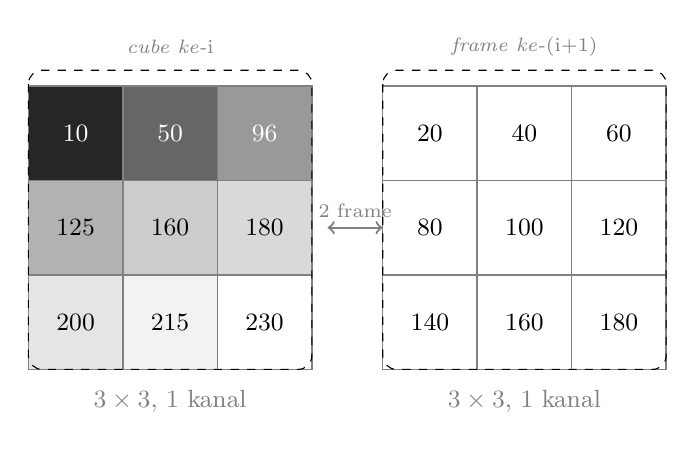
\begin{tikzpicture}[
  cell/.style={
    minimum width=12mm, minimum height=12mm,
    draw=black!50, line width=0.5pt,
    align=center, font=\small
  }
]

% ================= FRAME 1 =================
%\node[font=\small\bfseries] at (1.8,2) {Frame 1 (grayscale)};

% baris 1
\node[cell, fill=black!85, text=white] at (0,0) {10};
\node[cell, fill=black!60, text=white] at (1.2,0) {50};
\node[cell, fill=black!40, text=white] at (2.4,0) {96};

% baris 2
\node[cell, fill=black!30] at (0,-1.2) {125};
\node[cell, fill=black!20] at (1.2,-1.2) {160};
\node[cell, fill=black!15] at (2.4,-1.2) {180};

% baris 3
\node[cell, fill=black!10] at (0,-2.4) {200};
\node[cell, fill=black!5]  at (1.2,-2.4) {215};
\node[cell, fill=white]    at (2.4,-2.4) {230};

% border frame 1
\draw[dashed, rounded corners=5pt]
(-0.6,0.8) rectangle (3,-3);

\node[font=\scriptsize, gray] at (1.2,1.1) {\textit{cube ke-}i};
\node[font=\small, gray] at (1.2,-3.4) {$3\times3$, 1 kanal};

% ================= FRAME 2 =================
%\node[font=\small\bfseries] at (6,2) {Frame 2 (grayscale)};

\foreach \val/\r/\c in {
  20/0/0, 40/0/1, 60/0/2,
  80/1/0,100/1/1,120/1/2,
 140/2/0,160/2/1,180/2/2}
{
  \node[cell, fill=white] at (\c*1.2+4.5, -\r*1.2) {\val};
}

% border frame 2
\draw[dashed, rounded corners=5pt]
(3.9,0.8) rectangle (7.5,-3);

\node[font=\scriptsize, gray] at (5.7,1.1) {\textit{frame ke-}(i+1)};
\node[font=\small, gray] at (5.7,-3.4) {$3\times3$, 1 kanal};

% ================= ARROW =================
\draw[<->, thick, gray]
(3.2,-1.2) -- node[above, font=\scriptsize]{2 frame} (3.9,-1.2);

\end{tikzpicture}
}

\caption{Contoh \textit{spatio-temporal cube} berisi 2 frame berukuran $3\times3$ piksel (disederhanakan dari $2\times16\times16$).}
\label{fig:cube_example}
\end{figure}


\subsubsection{Flatten Tubelet}
 
Setiap cube ke-$i$ berbentuk $\mathbb{R}^{t\times p\times p\times C}$
diluruskan menjadi vektor satu dimensi dengan membaca piksel secara
berurutan: kanal $\to$ kolom $\to$ baris $\to$ frame.
Untuk contoh $3\times3$ grayscale ($C=1$):
 
\vspace{0.5cm}
\begin{equation}
  \mathbf{x}_i^{\text{flat}} \in
  \mathbb{R}^{t\cdot p\cdot p\cdot C}
  = \mathbb{R}^{2\times3\times3\times1}
  = \mathbb{R}^{18}
\end{equation}
\myequations{Dimensi vektor hasil flattening cube}
\vspace{0.5cm}
 
\noindent
Menggunakan nilai piksel dari Gambar~\ref{fig:cube_example},
proses \textit{flatten} menghasilkan vektor berikut.
Frame~1 dibaca terlebih dahulu baris per baris dari kiri ke kanan,
kemudian Frame~2 dengan urutan yang sama:
 
\vspace{0.5cm}
\begin{equation}
  \mathbf{x}_i^{\text{flat}}
  = \scalebox{0.80}{\ensuremath{%
      [\underbrace{10,\;50,\;96,\;125,\;160,\;180,\;200,\;215,\;230}_{%
         \text{Frame 1: baris 0, 1, 2}},\;
       \underbrace{20,\;40,\;60,\;80,\;100,\;120,\;140,\;160,\;180}_{%
         \text{Frame 2: baris 0, 1, 2}}]}}
\end{equation}
\myequations{Representasi vektor flattening cube}
\vspace{0.5cm}
 
\noindent
Tidak ada operasi matematika dalam proses \textit{flatten} ini, nilai
piksel tidak berubah, hanya posisi dalam memori yang diluruskan dari
susunan 3D menjadi satu baris lurus sepanjang 18 elemen.
Pada data sesungguhnya dengan patch $16\times16$ dan RGB ($C=3$),
panjang vektor menjadi:
 
\vspace{0.5cm}
\begin{align*}
  |\mathbf{x}_i^{\text{flat}}|
  &= 2 \times 16 \times 16 \times 3 \notag \\
  &= 1{.}536 \text{ elemen}
\end{align*}
\vspace{0.5cm}
 
\begin{figure}[h!]
\centering
\resizebox{0.80\linewidth}{!}{%
\fbox{%
\begin{tikzpicture}[
  cell/.style={minimum width=10mm, minimum height=9mm,
    draw=black!40, line width=0.4pt, align=center, font=\tiny},
  fcell/.style={minimum width=10mm, minimum height=9mm,
    draw=black!40, line width=0.4pt, align=center, font=\tiny},
  arr/.style={-{Stealth[length=4pt]}, line width=0.7pt, gray!60}
]
  \node[font=\small\bfseries] at (1.6, 1.6) {Cube $i$};
  \foreach \val/\bg/\r/\c in {
    10/frame1color/0/0, 50/frame1color/0/1, 96/frame1color/0/2,
   125/frame1color/1/0,160/frame1color/1/1,180/frame1color/1/2,
   200/frame1color/2/0,215/frame1color/2/1,230/frame1color/2/2}
  { \node[cell, fill=\bg] at (\c*1.05+0.55, -\r*1.0+0.65) {\val}; }
  \foreach \val/\bg/\r/\c in {
    20/frame2color/0/0, 40/frame2color/0/1, 60/frame2color/0/2,
    80/frame2color/1/0,100/frame2color/1/1,120/frame2color/1/2,
   140/frame2color/2/0,160/frame2color/2/1,180/frame2color/2/2}
  { \node[cell, fill=\bg] at (\c*1.05+0.55+0.3, -\r*1.0+0.65-0.3) {\val}; }
  \node[font=\tiny, frame1color!80!black] at (0.1, 0.65) {F1};
  \node[font=\tiny, frame2color!80!black] at (0.4, 0.35) {F2};
  \draw[arr, line width=1pt] (3.7, 0.2) --
    node[above, font=\small]{flatten} (5.0, 0.2);
  \node[font=\small\bfseries] at (8.5, 1.6) {Vektor flat $\mathbf{x}_i^{\text{flat}}$};
  \foreach \val/\bg/\idx in {
    10/frame1color/0, 50/frame1color/1,  96/frame1color/2,
   125/frame1color/3,160/frame1color/4, 180/frame1color/5,
   200/frame1color/6,215/frame1color/7, 230/frame1color/8,
    20/frame2color/9, 40/frame2color/10, 60/frame2color/11,
    80/frame2color/12,100/frame2color/13,120/frame2color/14,
   140/frame2color/15,160/frame2color/16,180/frame2color/17}
  {
    \pgfmathsetmacro{\col}{mod(\idx,9)}
    \pgfmathsetmacro{\row}{int(\idx/9)}
    \node[fcell, fill=\bg] at (\col*1.05+5.55, -\row*1.05+0.65) {\val};
  }
  \draw[decorate, decoration={brace,amplitude=5pt}]
    (5.05, -1.45) -- (14.45, -1.45)
    node[midway, below=6pt, font=\scriptsize]
    {18 elemen ($= 2\times3\times3\times1$, contoh 3$\times$3 grayscale)};
  \foreach \idx in {0,...,17} {
    \pgfmathsetmacro{\col}{mod(\idx,9)}
    \pgfmathsetmacro{\row}{int(\idx/9)}
    \node[font=\tiny, gray!60]
      at (\col*1.05+5.55, -\row*1.05+1.1)
      {$x_{\pgfmathprintnumber[fixed]{\idx}}$};
  }
\end{tikzpicture}
}%
}
\caption{Proses \textit{flatten} cube ke-$i$. Frame~1
         (\colorbox{frame1color}{\strut F1}) dibaca terlebih dahulu,
         diikuti Frame~2 (\colorbox{frame2color}{\strut F2}),
         menghasilkan vektor $\mathbf{x}_i^{\text{flat}} \in \mathbb{R}^{18}$.}
\label{fig:flatten}
\end{figure}
 
 
\subsubsection{Proyeksi Linear (Patch Embedding)}
 
Vektor $\mathbf{x}_i^{\text{flat}} \in \mathbb{R}^{1536}$ diproyeksikan
ke dimensi embedding $d=384$ melalui perkalian matriks bobot
$\mathbf{W}_E$:
 
\vspace{0.5cm}
\begin{equation}
  \mathbf{e}_i = \mathbf{W}_E\,\mathbf{x}_i^{\text{flat}} + \mathbf{b}_E
\end{equation}
\myequations{Proyeksi linear patch embedding}
\vspace{0.5cm}

\noindent
dengan $\mathbf{W}_E \in \mathbb{R}^{384\times1536}$ dan $\mathbf{b}_E \in \mathbb{R}^{384}$.
\vspace{0.5cm}
 
\noindent
Untuk memahami cara kerjanya, berikut ditampilkan contoh perhitungan
menggunakan vektor flat $\mathbf{x}^{\text{flat}} \in \mathbb{R}^{18}$
dari contoh 3$\times$3 di atas, dengan matriks $\mathbf{W}_E$
berukuran $4\times18$ (disederhanakan menjadi 4 dimensi output):
 
\vspace{0.5cm}
\begin{equation*}
  \mathbf{x}^{\text{flat}}
  = \scalebox{0.82}{\ensuremath{%
      [10,\;50,\;96,\;125,\;160,\;180,\;200,\;215,\;230,\;
       20,\;40,\;60,\;80,\;100,\;120,\;140,\;160,\;180]}}
\end{equation*}
\vspace{0.5cm}
 
\noindent
Misalkan baris pertama matriks $\mathbf{W}_E$ adalah:
 
\vspace{0.5cm}
\begin{multline*}
  \mathbf{w}_{E,1}
  = [0.02,\;{-0.01},\;0.03,\;{-0.02},\;0.01,\;{-0.03},\;
     0.02,\;0.01,\;{-0.02}, \\
     0.03,\;{-0.01},\;0.02,\;{-0.01},\;0.03,\;{-0.02},\;
     0.01,\;0.02,\;{-0.01}]
\end{multline*}
\vspace{0.5cm}
 
\noindent
Elemen pertama dari $\mathbf{e}_i$ diperoleh dari perkalian titik
(\textit{dot product}) antara $\mathbf{w}_{E,1}$ dan
$\mathbf{x}^{\text{flat}}$:
 
\vspace{0.5cm}
\begin{align*}
  e_{i,1}
  &= \mathbf{w}_{E,1} \cdot \mathbf{x}^{\text{flat}} + b_{E,1}
  \notag \\
  &= (0.02\times10) + (-0.01\times50) + (0.03\times96) \notag \\
  &\qquad + (-0.02\times125) + (0.01\times160) + (-0.03\times180)
  \notag \\
  &\quad + (0.02\times200) + (0.01\times215) + (-0.02\times230) \notag \\
  &\qquad + (0.03\times20) + (-0.01\times40) + (0.02\times60)
  \notag \\
  &\quad + (-0.01\times80) + (0.03\times100) + (-0.02\times120) \notag \\
  &\qquad + (0.01\times140) + (0.02\times160) + (-0.01\times180) + 0
  \notag \\[4pt]
  &= 0.20 + (-0.50) + 2.88 + (-2.50) + 1.60 + (-5.40)
  \notag \\
  &\quad + 4.00 + 2.15 + (-4.60) + 0.60 + (-0.40) + 1.20
  \notag \\
  &\quad + (-0.80) + 3.00 + (-2.40) + 1.40 + 3.20 + (-1.80)
  \notag \\[4pt]
  &= (0.20 - 0.50 + 2.88 - 2.50 + 1.60 - 5.40)
  \notag \\
  &\quad + (4.00 + 2.15 - 4.60 + 0.60 - 0.40 + 1.20)
  \notag \\
  &\quad + (-0.80 + 3.00 - 2.40 + 1.40 + 3.20 - 1.80)
  \notag \\[4pt]
  &= (-3.72) + (2.95) + (2.60)
  \notag \\[4pt]
  &= \mathbf{1.83}
\end{align*}
\vspace{0.5cm}
 
\noindent
Proses yang sama dilakukan untuk seluruh 384 baris matriks
$\mathbf{W}_E$ sehingga menghasilkan vektor embedding lengkap
$\mathbf{e}_i \in \mathbb{R}^{384}$.
Jumlah parameter pada lapisan ini adalah:
 
\vspace{0.5cm}
\begin{align*}
  |\mathbf{W}_E| + |\mathbf{b}_E|
  &= (384 \times 1536) + 384 \notag \\
  &= 589.824 + 384 \notag \\
  &= 590{.}208 \text{ parameter}
\end{align*}
\vspace{0.5cm}
 
\begin{figure}[h!]
\centering
\resizebox{0.75\linewidth}{!}{%
\fbox{%
\begin{tikzpicture}[scale=0.7,
  arr/.style={-{Stealth[length=4pt]}, line width=0.7pt, gray!60},
  box/.style={rectangle, rounded corners=3pt,
              draw=black!40, line width=0.5pt,
              minimum width=18mm, align=center, font=\small}
]
  \foreach \v/\bg/\i in {
    10/frame1color/0,50/frame1color/1,96/frame1color/2,
    {$\vdots$}/{white}/3,180/frame1color/4,
    20/frame2color/5,{$\vdots$}/{white}/6,180/frame2color/7}
  { \node[minimum width=12mm, minimum height=7mm,
          draw=black!30, fill=\bg, align=center, font=\tiny]
      at (0, -\i*0.72+2.5) {\v}; }
  \node[font=\scriptsize, gray] at (0, -7*0.72+2.5-0.6) {$\mathbb{R}^{1536}$};
  \node[font=\small\bfseries] at (0, 3.1) {$\mathbf{x}_i^{\text{flat}}$};
  \foreach \r in {0,...,4} {
    \foreach \c in {0,...,7} {
      \node[minimum width=5.5mm, minimum height=5.5mm,
            draw=black!20, fill=embedcolor!50, align=center, font=\tiny]
        at (\c*0.56+2.4, -\r*0.56+1.4) {$w$}; } }
  \node[font=\scriptsize, gray] at (4.36, -3.0+1.4-0.55) {$\mathbb{R}^{384\times1536}$};
  \node[font=\small\bfseries] at (4.36, 2.0) {$\mathbf{W}_E$};
  \node[font=\large] at (1.5, 0.5) {$\times$};
  \node[font=\large] at (6.8, 0.5) {$=$};
  \foreach \v/\i in {1.83/0,{-0.47}/1,0.92/2,
                     {$\vdots$}/3,1.15/4,{$\vdots$}/5,
                     {-0.33}/6,0.74/7}
  { \node[minimum width=14mm, minimum height=7mm,
          draw=black!30, fill=embedcolor!70, align=center, font=\tiny]
      at (7.9, -\i*0.72+2.5) {\v}; }
  \node[font=\scriptsize, gray] at (7.9, -7*0.72+2.5-0.6) {$\mathbb{R}^{384}$};
  \node[font=\small\bfseries] at (7.9, 3.1) {$\mathbf{e}_i$};
\end{tikzpicture}
}}
\caption{Proyeksi linear (\textit{patch embedding}): vektor flat
         $\mathbf{x}_i^{\text{flat}}\in\mathbb{R}^{1536}$ dikalikan
         $\mathbf{W}_E\in\mathbb{R}^{384\times1536}$ menghasilkan
         $\mathbf{e}_i\in\mathbb{R}^{384}$.}
\label{fig:patch_embed}
\end{figure}
 
 
\subsubsection{Positional Embedding}
 
Karena Transformer tidak memiliki kesadaran posisi secara bawaan,
vektor posisi $\mathbf{p}_i \in \mathbb{R}^{384}$ yang dapat dilatih
ditambahkan ke setiap token embedding:
 
\vspace{0.5cm}
\begin{equation}
  \mathbf{z}_i^{(0)} = \mathbf{e}_i + \mathbf{p}_i,
  \qquad i = 1,2,\ldots,N
\end{equation}
\myequations{Penambahan positional embedding pada token}
\vspace{0.5cm}
 
\noindent
Penambahan ini dilakukan secara elemen-per-elemen.
Sebagai contoh, misalkan 4 elemen pertama dari $\mathbf{e}_i$ dan
$\mathbf{p}_i$ adalah:
 
\vspace{0.5cm}
\begin{align*}
  \mathbf{e}_i^{(1:4)}   &= [\;1.83,\; -0.47,\; 0.92,\; 1.15\;] \\[4pt]
  \mathbf{p}_i^{(1:4)}   &= [\;0.10,\;\;\; 0.05,\; {-0.08},\; 0.12\;]
\end{align*}
\vspace{0.5cm}
 
\noindent
Maka 4 elemen pertama token awal $\mathbf{z}_i^{(0)}$ adalah:
 
\vspace{0.5cm}
\begin{align*}
  z_{i,1}^{(0)} &= 1.83 + 0.10 = \mathbf{1.93} \\[3pt]
  z_{i,2}^{(0)} &= -0.47 + 0.05 = \mathbf{-0.42} \\[3pt]
  z_{i,3}^{(0)} &= 0.92 + (-0.08) = \mathbf{0.84} \\[3pt]
  z_{i,4}^{(0)} &= 1.15 + 0.12 = \mathbf{1.27}
\end{align*}
\vspace{0.5cm}
 
\noindent
Proses yang sama diterapkan pada seluruh 384 elemen, sehingga
$\mathbf{z}_i^{(0)} \in \mathbb{R}^{384}$.
Keseluruhan $N=1568$ token awal membentuk matriks:
 
\vspace{0.5cm}
\begin{equation}
  \mathbf{Z}^{(0)}
  = \bigl[\mathbf{z}_1^{(0)},\ldots,\mathbf{z}_{1568}^{(0)}\bigr]
  \in \mathbb{R}^{1568\times384}
\end{equation}
\myequations{Matriks token awal encoder}
\vspace{0.5cm}
 
\begin{figure}[h!]
\centering
\resizebox{0.65\linewidth}{!}{%
\fbox{%
\begin{tikzpicture}[scale=0.7,
  arr/.style={-{Stealth[length=4pt]}, line width=0.7pt, gray!60},
  vec/.style={minimum width=14mm, minimum height=7mm,
              draw=black!30, align=center, font=\tiny}
]
  \node[font=\small\bfseries] at (0,2.2) {$\mathbf{e}_i$};
  \foreach \v/\bg/\i in {
    1.83/embedcolor/0,{-0.47}/embedcolor/1,
    0.92/embedcolor/2,{$\vdots$}/white/3,1.15/embedcolor/4}
  { \node[vec, fill=\bg!70] at (0,-\i*0.75+1.5) {\v}; }
  \node[font=\scriptsize,gray] at (0,-4*0.75+1.5-0.5) {$\mathbb{R}^{384}$};
  \node[font=\Large] at (1.5, 0.375) {$+$};
  \node[font=\small\bfseries] at (3,2.2) {$\mathbf{p}_i$};
  \foreach \v/\bg/\i in {
    0.10/poscolor/0,0.05/poscolor/1,
    {-0.08}/poscolor/2,{$\vdots$}/white/3,0.12/poscolor/4}
  { \node[vec, fill=\bg!70] at (3,-\i*0.75+1.5) {\v}; }
  \node[font=\scriptsize,gray] at (3,-4*0.75+1.5-0.5) {$\mathbb{R}^{384}$};
  \node[font=\Large] at (4.5, 0.375) {$=$};
  \node[font=\small\bfseries] at (6,2.2) {$\mathbf{z}_i^{(0)}$};
  \foreach \v/\bg/\i in {
    1.93/tokencolor/0,{-0.42}/tokencolor/1,
    0.84/tokencolor/2,{$\vdots$}/white/3,1.27/tokencolor/4}
  { \node[vec, fill=\bg!70] at (6,-\i*0.75+1.5) {\v}; }
  \node[font=\scriptsize,gray] at (6,-4*0.75+1.5-0.5) {$\mathbb{R}^{384}$};
  \node[font=\scriptsize, align=center, gray] at (3, -3.5)
    {$\mathbf{p}_i$ menyandikan posisi temporal-spasial\\
     token ke-$i$: indeks waktu, baris, dan kolom};
\end{tikzpicture}
}}
\caption{Penambahan \textit{positional embedding} $\mathbf{p}_i$ secara
         \textit{additive} ke token embedding $\mathbf{e}_i$
         menghasilkan token awal $\mathbf{z}_i^{(0)} \in \mathbb{R}^{384}$.}
\label{fig:pos_embed}
\end{figure}
 
 
% ============================================================
\subsection{Encoder ViT-S}
% ============================================================
 
Encoder terdiri atas $L=12$ \textit{Transformer block} identik.
Konfigurasi ViT-S dirangkum pada Tabel~\ref{tab:vits_config}.
 
\begin{table}[h!]
\centering
\caption{Konfigurasi Hiperparameter ViT-S}
\label{tab:vits_config}
\begin{tabular}{lcc}
\hline
Hiperparameter & Notasi & Nilai \\
\hline
Dimensi embedding        & $d$      & 384  \\
Jumlah block             & $L$      & 12   \\
Jumlah head              & $h$      & 6    \\
Dimensi per head         & $d_h$    & 64   \\
Rasio ekspansi FFN       & $r$      & 4    \\
Dimensi FFN              & $d_{ff}$ & 1536 \\
Aktivasi                 & -        & GELU \\
Normalisasi              & -        & LayerNorm \\
\hline
\end{tabular}
\end{table}
 
\begin{figure}[h!]
\centering
\resizebox{0.60\linewidth}{!}{%
\fbox{%
\begin{tikzpicture}[scale=0.7,
  node distance=6mm and 10mm,
  blk/.style={rectangle, rounded corners=4pt,
              minimum width=44mm, minimum height=10mm,
              draw=black!40, line width=0.5pt,
              align=center, font=\small},
  add/.style={circle, draw=black!50, minimum size=7mm,
              font=\small, line width=0.5pt},
  arr/.style={-{Stealth[length=4pt]}, line width=0.6pt}
]
  \node[blk, fill=frame1color!40]  (in)   {$\mathbf{Z}^{(\ell-1)} \in \mathbb{R}^{N\times384}$};
  \node[blk, fill=gray!15, below=of in]  (ln1)  {Layer Norm};
  \node[blk, fill=attncolor!50, below=of ln1] (mhsa) {Multi-Head Self-Attention\\$h=6,\;d_h=64$};
  \node[add, below=of mhsa]        (add1) {$+$};
  \node[blk, fill=gray!15, below=of add1] (ln2)  {Layer Norm};
  \node[blk, fill=ffncolor!60, below=of ln2] (ffn)  {Feed-Forward Network\\$d_{ff}=1536$, GELU};
  \node[add, below=of ffn]         (add2) {$+$};
  \node[blk, fill=outcolor!50, below=of add2]  (out)  {$\mathbf{Z}^{(\ell)} \in \mathbb{R}^{N\times384}$};
  \draw[arr] (in)--(ln1); \draw[arr] (ln1)--(mhsa);
  \draw[arr] (mhsa)--(add1); \draw[arr] (add1)--(ln2);
  \draw[arr] (ln2)--(ffn); \draw[arr] (ffn)--(add2);
  \draw[arr] (add2)--(out);
  \draw[arr, dashed, gray!70]
    (in.east) -- ++(1.2,0) |- node[right, font=\scriptsize, gray]{residual} (add1.east);
  \draw[arr, dashed, gray!70]
    (add1.west) -- ++(-1.2,0) |- node[left, font=\scriptsize, gray]{residual} (add2.west);
  \node[font=\small, gray, right=15mm of out] {$\times\; L=12$};
\end{tikzpicture}
}}
\caption{Satu \textit{Transformer block} pada encoder ViT-S.
         Block ini diulang $L=12$ kali secara berurutan.}
\label{fig:transformer_block}
\end{figure}
 
 
\subsubsection{Perhitungan Layer Normalization}
 
Sebelum masuk ke operasi \textit{attention}, setiap token dinormalisasi
menggunakan Layer Normalization. Normalisasi ini menstabilkan distribusi
nilai di dalam vektor token sehingga proses optimasi berjalan lebih
konsisten.
 
\vspace{0.5cm}
\begin{align}
  \mathrm{LN}(\mathbf{z})
  &= \boldsymbol{\gamma} \odot
    \frac{\mathbf{z}-\mu_z}{\sqrt{\sigma_z^2+\epsilon}}
    + \boldsymbol{\beta} \notag \\
  \mu_z &= \frac{1}{d}\sum_k z_k,\qquad
  \sigma_z^2 = \frac{1}{d}\sum_k(z_k-\mu_z)^2
\end{align}
\myequations{Layer normalization pada token}
\vspace{0.5cm}
 
\noindent
Berikut adalah perhitungan lengkap menggunakan token
$\mathbf{z}^{(0)} = [1.93,\;-0.42,\;0.84,\;1.27]$
(disingkat 4 dimensi untuk kemudahan ilustrasi):
 
\vspace{0.5cm}
\noindent Langkah 1: Hitung rata-rata elemen token:
 
\vspace{0.5cm}
\begin{align*}
  \mu_z
  &= \frac{1}{4}(z_1 + z_2 + z_3 + z_4) \notag \\
  &= \frac{1}{4}(1.93 + (-0.42) + 0.84 + 1.27) \notag \\
  &= \frac{3.62}{4} \notag \\
  &= 0.905
\end{align*}
\vspace{0.5cm}
 
\noindent Langkah 2: Hitung variansi elemen token:
 
\vspace{0.5cm}
\begin{align*}
  \sigma_z^2
  &= \frac{1}{4}\bigl[(1.93-0.905)^2 + (-0.42-0.905)^2
     + (0.84-0.905)^2 + (1.27-0.905)^2\bigr] \notag \\
  &= \frac{1}{4}\bigl[(1.025)^2 + (-1.325)^2 + (-0.065)^2 + (0.365)^2\bigr] \notag \\
  &= \frac{1}{4}(1.051 + 1.756 + 0.004 + 0.133) \notag \\
  &= \frac{2.944}{4} \notag \\
  &= 0.736
\end{align*}
\vspace{0.5cm}
 
\noindent Langkah 3: Normalisasi setiap elemen:
 
\vspace{0.5cm}
\begin{align*}
  \hat{z}_1 &= \frac{1.93 - 0.905}{\sqrt{0.736 + 10^{-6}}}
             = \frac{1.025}{0.858} = \mathbf{1.195} \\[4pt]
  \hat{z}_2 &= \frac{-0.42 - 0.905}{0.858}
             = \frac{-1.325}{0.858} = \mathbf{-1.544} \\[4pt]
  \hat{z}_3 &= \frac{0.84 - 0.905}{0.858}
             = \frac{-0.065}{0.858} = \mathbf{-0.076} \\[4pt]
  \hat{z}_4 &= \frac{1.27 - 0.905}{0.858}
             = \frac{0.365}{0.858} = \mathbf{0.425}
\end{align*}
\vspace{0.5cm}
 
\noindent Langkah 4: Terapkan parameter scale dan shift:
 
\vspace{0.5cm}
\noindent
Misalkan $\boldsymbol{\gamma} = [1.0, 1.0, 1.0, 1.0]$ dan
$\boldsymbol{\beta} = [0.0, 0.0, 0.0, 0.0]$ (nilai awal tipikal):
 
\vspace{0.5cm}
\begin{align*}
  \mathrm{LN}(\mathbf{z})
  = \boldsymbol{\gamma} \odot \hat{\mathbf{z}} + \boldsymbol{\beta}
  = [\mathbf{1.195},\; \mathbf{-1.544},\; \mathbf{-0.076},\; \mathbf{0.425}]
\end{align*}
\vspace{0.5cm}
 
\noindent
Perhatikan bahwa rata-rata hasil normalisasi mendekati nol:
$(1.195 - 1.544 - 0.076 + 0.425)/4 = 0/4 = 0.000$,
dan standar deviasinya mendekati satu, yang merupakan tujuan
dari Layer Normalization.
 
 
\subsubsection{Perhitungan Multi-Head Self-Attention (MHSA)}
 
\vspace{0.5cm}
\begin{align}
  \mathbf{Q} &= \mathbf{Z}\mathbf{W}^Q,\quad
  \mathbf{K} = \mathbf{Z}\mathbf{W}^K,\quad
  \mathbf{V} = \mathbf{Z}\mathbf{W}^V \notag \\
  &\text{dengan}\quad \mathbf{W}^Q,\mathbf{W}^K,\mathbf{W}^V \in \mathbb{R}^{384\times384}
\end{align}
\myequations{Transformasi Query, Key, dan Value}
\vspace{0.5cm}
 
\noindent
Kemudian dibagi ke $h=6$ kepala, masing-masing berdimensi $d_h = 384/6 = 64$.
 
\begin{figure}[h!]
\centering
\resizebox{0.80\linewidth}{!}{%
\fbox{%
\begin{tikzpicture}[
  arr/.style={-{Stealth[length=4pt]}, line width=0.6pt, gray!70},
  tok/.style={minimum width=12mm, minimum height=8mm,
              draw=black!30, align=center, font=\tiny, rounded corners=2pt},
  head/.style={minimum width=14mm, minimum height=7mm,
               draw=black!30, align=center, font=\tiny, rounded corners=2pt}
]
  \node[font=\small\bfseries] at (0, 3.5) {Token input ($N$ token)};
  \foreach \lbl/\bg/\i in {
    {$\mathbf{z}_1$}/tokencolor/0,
    {$\mathbf{z}_2$}/tokencolor/1,
    {$\vdots$}/white/2,
    {$\mathbf{z}_N$}/tokencolor/3}
  { \node[tok, fill=\bg!60] at (0, -\i*1.0+2.5) {\lbl}; }
  \draw[arr] (0.7, 0.75) -- (2.0, 1.8) node[midway, above, font=\tiny]{$\mathbf{W}^Q$};
  \draw[arr] (0.7, 0.75) -- (2.0, 0.75) node[midway, above, font=\tiny]{$\mathbf{W}^K$};
  \draw[arr] (0.7, 0.75) -- (2.0,-0.3) node[midway, below, font=\tiny]{$\mathbf{W}^V$};
  \node[tok, fill=attncolor!50, minimum width=18mm] at (3.0, 1.8)
    {$\mathbf{Q}\in\mathbb{R}^{N\times384}$};
  \node[tok, fill=attncolor!30, minimum width=18mm] at (3.0, 0.75)
    {$\mathbf{K}\in\mathbb{R}^{N\times384}$};
  \node[tok, fill=attncolor!20, minimum width=18mm] at (3.0,-0.3)
    {$\mathbf{V}\in\mathbb{R}^{N\times384}$};
  \node[font=\scriptsize, gray] at (5.2, 2.5) {dibagi $h=6$ kepala ($d_h=64$)};
  \foreach \m/\y in {1/2.0, 2/1.2, 3/0.4, 4/-0.4}
  { \node[head, fill=attncolor!40] at (5.8, \y)
      {head$_{\m}$\\$\mathbb{R}^{N\times64}$};
    \draw[arr] (4.0, 1.0) -- (5.1, \y); }
  \node[font=\tiny, gray] at (5.8, -1.0) {$\vdots$ (6 total)};
  \draw[arr] (6.55, 0.8) -- (7.5, 0.8);
  \node[tok, fill=embedcolor!60, minimum width=22mm] at (8.8, 0.8)
    {concat $\to$ $\times\mathbf{W}^O$\\$\mathbb{R}^{N\times384}$};
  \node[font=\scriptsize, gray] at (8.8, 0.0)
    {$\mathbf{W}^O\in\mathbb{R}^{384\times384}$};
\end{tikzpicture}
}%
}
\caption{Alur \textit{Multi-Head Self-Attention}: $\mathbf{Q}$, $\mathbf{K}$,
         $\mathbf{V}$ dibagi ke $h=6$ kepala berdimensi $d_h=64$,
         hasilnya digabung dan diproyeksikan kembali ke $\mathbb{R}^{384}$.}
\label{fig:mhsa}
\end{figure}
 
\vspace{0.5cm}
\noindent Perhitungan Scaled Dot-Product Attention\par
\vspace{0.3cm}
 
\noindent
Untuk satu kepala, misalkan terdapat 4 token ($N=4$) dengan dimensi
per kepala $d_h=2$ (disederhanakan). Vektor Query dan Key dari
keempat token adalah:
 
\vspace{0.5cm}
\begin{align*}
  \mathbf{Q}^{(m)}
  &= \begin{bmatrix}
       0.5 & 0.3 \\
       0.7 & -0.2 \\
       0.2 & 0.8 \\
       0.6 & 0.1
     \end{bmatrix}, \notag \\[6pt]
  \mathbf{K}^{(m)}
  &= \begin{bmatrix}
       0.4 & 0.2 \\
       0.9 & 0.1 \\
       -0.3 & 0.8 \\
       0.6 & 0.5
     \end{bmatrix}
\end{align*}
\vspace{0.5cm}
 
\noindent Langkah 1: Hitung matriks skor mentah
$\mathbf{Q}^{(m)}\bigl(\mathbf{K}^{(m)}\bigr)^\top$:
 
\vspace{0.5cm}
\begin{align}
  \mathbf{S} &= \mathbf{Q}^{(m)}\bigl(\mathbf{K}^{(m)}\bigr)^\top \notag \\[4pt]
  &= \scalebox{0.70}{\ensuremath{\begin{bmatrix}
       (0.5)(0.4)+(0.3)(0.2) & (0.5)(0.9)+(0.3)(0.1)
         & (0.5)(-0.3)+(0.3)(0.8) & (0.5)(0.6)+(0.3)(0.5) \\
       (0.7)(0.4)+(-0.2)(0.2) & (0.7)(0.9)+(-0.2)(0.1)
         & (0.7)(-0.3)+(-0.2)(0.8) & (0.7)(0.6)+(-0.2)(0.5) \\
       (0.2)(0.4)+(0.8)(0.2) & (0.2)(0.9)+(0.8)(0.1)
         & (0.2)(-0.3)+(0.8)(0.8) & (0.2)(0.6)+(0.8)(0.5) \\
       (0.6)(0.4)+(0.1)(0.2) & (0.6)(0.9)+(0.1)(0.1)
         & (0.6)(-0.3)+(0.1)(0.8) & (0.6)(0.6)+(0.1)(0.5)
     \end{bmatrix}}} \notag \\[6pt]
  &= \begin{bmatrix}
       0.26 & 0.48 & 0.09 & 0.45 \\
       0.24 & 0.61 & -0.37 & 0.32 \\
       0.24 & 0.26 & 0.58 & 0.52 \\
       0.26 & 0.55 & -0.10 & 0.41
     \end{bmatrix}
\end{align}
\myequations{Perhitungan matriks skor mentah attention}
\vspace{0.5cm}
 
\noindent Langkah 2: Bagi dengan $\sqrt{d_h} = \sqrt{2} \approx 1.414$:
 
\vspace{0.5cm}
\begin{align*}
  \frac{\mathbf{S}}{\sqrt{d_h}}
  &= \frac{1}{1.414}
     \begin{bmatrix}
       0.26 & 0.48 & 0.09 & 0.45 \\
       0.24 & 0.61 & -0.37 & 0.32 \\
       0.24 & 0.26 & 0.58 & 0.52 \\
       0.26 & 0.55 & -0.10 & 0.41
     \end{bmatrix} \notag \\[6pt]
  &= \begin{bmatrix}
      0.184 & 0.339 & 0.064 & 0.318 \\
      0.170 & 0.431 & -0.262 & 0.226 \\
      0.170 & 0.184 & 0.410 & 0.368 \\
      0.184 & 0.389 & -0.071 & 0.290
    \end{bmatrix}
\end{align*}
\vspace{0.5cm}
 
\noindent Langkah 3: Terapkan Softmax per baris untuk mendapatkan
bobot atensi $\mathbf{A}^{(m)}$:
 
\vspace{0.5cm}
\noindent
Untuk baris pertama $[0.184,\; 0.339,\; 0.064,\; 0.318]$:
 
\vspace{0.5cm}
\begin{align}
  e^{0.184} &= 1.202, \quad
  e^{0.339}  = 1.404, \quad
  e^{0.064}  = 1.066, \quad
  e^{0.318}  = 1.374 \notag \\
  \Sigma &= 1.202 + 1.404 + 1.066 + 1.374 = 5.046 \notag \\[4pt]
  \mathbf{A}^{(m)}_{1,\cdot}
  &= \left[\frac{1.202}{5.046},\;\frac{1.404}{5.046},\;
           \frac{1.066}{5.046},\;\frac{1.374}{5.046}\right]
   = [\mathbf{0.238},\; \mathbf{0.278},\; \mathbf{0.211},\; \mathbf{0.272}]
\end{align}
\myequations{Perhitungan bobot attention dengan softmax}
\vspace{0.5cm}
 
\noindent
Dengan cara yang sama untuk seluruh baris, diperoleh matriks atensi:
 
\vspace{0.5cm}
\begin{equation*}
  \mathbf{A}^{(m)} =
  \begin{bmatrix}
    0.238 & 0.278 & 0.211 & 0.272 \\
    0.238 & 0.385 & 0.153 & 0.253 \\
    0.228 & 0.231 & 0.299 & 0.281 \\
    0.239 & 0.295 & 0.186 & 0.268 \\
  \end{bmatrix}
\end{equation*}
\vspace{0.5cm}
 
\noindent
Interpretasinya: token ke-1 (baris pertama) memberikan perhatian
terbesar kepada token ke-2 (bobot 0.278), diikuti token ke-4 (0.272),
token ke-1 itu sendiri (0.238), dan token ke-3 mendapat perhatian
paling kecil (0.211).
 
\vspace{0.5cm}
\noindent Langkah 4: Hitung output sebagai jumlah tertimbang dari Value:
 
\vspace{0.5cm}
\noindent
Misalkan matriks Value adalah:
 
\vspace{0.5cm}
\begin{align*}
  \mathbf{V}^{(m)}
  = \begin{bmatrix}
      0.3 & 0.7 \\ 0.8 & -0.2 \\ -0.4 & 0.5 \\ 0.6 & 0.3
    \end{bmatrix}
\end{align*}
\vspace{0.5cm}
 
\noindent
Output untuk token ke-1:
 
\vspace{0.5cm}
\begin{align*}
  \mathrm{head}_{m,1}
  &= \mathbf{A}^{(m)}_{1,\cdot} \cdot \mathbf{V}^{(m)} \notag \\[4pt]
  \text{dim 1}
  &= 0.238(0.3) + 0.278(0.8) + 0.211(-0.4) + 0.272(0.6) \notag \\
  &= 0.071 + 0.222 - 0.084 + 0.163
   = \mathbf{0.372} \notag \\[4pt]
  \text{dim 2}
  &= 0.238(0.7) + 0.278(-0.2) + 0.211(0.5) + 0.272(0.3) \notag \\
  &= 0.167 - 0.056 + 0.106 + 0.082
   = \mathbf{0.299}
\end{align*}
\vspace{0.5cm}
 
\noindent
Sehingga $\mathrm{head}_{m,1} = [0.372,\; 0.299]$.
Proses ini diulang untuk semua $N=1568$ token dan semua $h=6$ kepala.
Setelah seluruh kepala selesai, hasilnya digabung (\textit{concatenate})
dan dikalikan dengan $\mathbf{W}^O$ untuk menghasilkan output MHSA
berukuran $\mathbb{R}^{N \times 384}$.
 
\vspace{0.5cm}
\noindent Perhitungan Residual Connection Pertama\par
\vspace{0.3cm}
 
\noindent
Output MHSA ditambahkan dengan token masukan (sebelum LayerNorm)
melalui \textit{residual connection}. Misalkan untuk token ke-1
(4 dimensi contoh):
 
\vspace{0.5cm}
\begin{align*}
  \mathbf{Z}'_1
  &= \mathbf{z}_1^{(\ell-1)} + \mathrm{MHSA}_1 \notag \\
  &= [1.93,\; -0.42,\; 0.84,\; 1.27]
   + [0.42,\; -0.18,\; 0.31,\; 0.25] \notag \\
  &= [1.93+0.42,\; -0.42+(-0.18),\; 0.84+0.31,\; 1.27+0.25] \notag \\
  &= [\mathbf{2.35},\; \mathbf{-0.60},\; \mathbf{1.15},\; \mathbf{1.52}]
\end{align*}
\vspace{0.5cm}
 
 
\subsubsection{Perhitungan Feed-Forward Network (FFN)}
 
\vspace{0.5cm}
\begin{equation}
  \mathrm{FFN}(\mathbf{z})
  = \mathbf{W}_2\,\mathrm{GELU}\!\bigl(\mathbf{W}_1\mathbf{z}+\mathbf{b}_1\bigr)
    +\mathbf{b}_2
\end{equation}
\myequations{Fungsi Feed-Forward Network pada encoder}
\vspace{0.5cm}

\noindent
dengan $\mathbf{W}_1\in\mathbb{R}^{1536\times 384}$ adalah matriks proyeksi ekspansi
dan $\mathbf{W}_2\in\mathbb{R}^{384\times 1536}$ adalah matriks proyeksi kontraksi.
\vspace{0.5cm}
 
\begin{equation}
  \mathrm{GELU}(x)
  = x\cdot\frac{1}{2}\!\left[1+\mathrm{erf}\!\left(\frac{x}{\sqrt{2}}\right)\right]
\end{equation}
\myequations{Fungsi aktivasi GELU}
\vspace{0.5cm}
 
\noindent
Berikut adalah perhitungan lengkap FFN menggunakan token $\mathbf{z}'$
hasil residual di atas (disederhanakan menjadi input 4 dimensi,
output 4 dimensi, ekspansi tengah 8 dimensi):
 
\vspace{0.5cm}
\noindent Langkah 1: Proyeksi Linear Pertama
($\mathbf{W}_1$, ekspansi $4\times$):
 
\vspace{0.5cm}
\noindent
Misalkan 2 baris pertama $\mathbf{W}_1$ (ukuran $8\times4$ contoh) adalah:
 
\vspace{0.5cm}
\begin{align*}
  h_1
  &= \mathbf{w}_{1,1} \cdot \mathbf{z}' + b_{1,1} \notag \\
  &= (0.3)(2.35) + (-0.1)(-0.60) \notag \\
  &\quad + (0.4)(1.15) + (-0.2)(1.52) + 0 \notag \\
  &= 0.705 + 0.060 + 0.460 + (-0.304) \notag \\
  &= \mathbf{0.921} \\[4pt]
  h_2
  &= (-0.2)(2.35) + (0.5)(-0.60) \notag \\
  &\quad + (-0.1)(1.15) + (0.3)(1.52) + 0 \notag \\
  &= -0.470 + (-0.300) + (-0.115) + 0.456 \notag \\
  &= \mathbf{-0.429}
\end{align*}
\vspace{0.5cm}
 
\noindent Langkah 2: Terapkan aktivasi GELU:
 
\vspace{0.5cm}
\noindent
GELU diaplikasikan elemen per elemen. Menggunakan aproksimasi:

\begin{multline*}
  \mathrm{GELU}(x) \approx \\
  0.5x\!\left(1 + \tanh\!\left(\sqrt{\tfrac{2}{\pi}}\,
  \bigl(x + 0{,}044715\,x^3\bigr)\right)\right)
\end{multline*}
 
\vspace{0.5cm}
\begin{align*}
  \text{Untuk } h_1 = 0.921: \notag \\
  0.044715 \times (0.921)^3
  &= 0.044715 \times 0.782 = 0.035 \notag \\
  \sqrt{2/\pi} \times (0.921 + 0.035)
  &= 0.7979 \times 0.956 = 0.763 \notag \\
  \tanh(0.763) &= 0.644 \notag \\
  \mathrm{GELU}(0.921)
  &= 0.5 \times 0.921 \times (1 + 0.644)
   = 0.5 \times 0.921 \times 1.644
   = \mathbf{0.757} \\[10pt]
  \text{Untuk } h_2 = -0.429: \notag \\
  0.044715 \times (-0.429)^3
  &= 0.044715 \times (-0.079) = -0.004 \notag \\
  \sqrt{2/\pi} \times (-0.429 + (-0.004))
  &= 0.7979 \times (-0.433) = -0.346 \notag \\
  \tanh(-0.346) &= -0.333 \notag \\
  \mathrm{GELU}(-0.429)
  &= 0.5 \times (-0.429) \times (1 + (-0.333))
   = 0.5 \times (-0.429) \times 0.667
   = \mathbf{-0.143}
\end{align*}
\vspace{0.5cm}
 
\noindent
Nilai positif besar ($h_1=0.921$) hampir tidak berubah setelah GELU
($0.757$), sedangkan nilai negatif ($h_2=-0.429$) diredam menjadi
lebih kecil ($-0.143$). Ini berbeda dengan ReLU yang langsung memangkas
nilai negatif menjadi tepat nol.
 
\vspace{0.5cm}
\noindent Langkah 3: Proyeksi Linear Kedua ($\mathbf{W}_2$, kompresi kembali):
 
\vspace{0.5cm}
\noindent
Misalkan output elemen pertama setelah $\mathbf{W}_2$:
 
\vspace{0.5cm}
\begin{align*}
  \mathrm{FFN}_1(\mathbf{z}')
  &= (0.4)(0.757) + (-0.3)(-0.143) + \ldots + b_{2,1} \notag \\
  &= 0.303 + 0.043 + \ldots \notag \\
  &= \mathbf{0.512} \quad \text{(contoh hasil elemen pertama)}
\end{align*}
\vspace{0.5cm}
 
\vspace{0.5cm}
\noindent Perhitungan Residual Connection Kedua dan Satu Block Lengkap\par
\vspace{0.3cm}
 
\noindent
Output FFN ditambahkan kembali ke $\mathbf{Z}'$ melalui residual
connection kedua. Misalkan untuk token ke-1 (4 dimensi contoh):
 
\vspace{0.5cm}
\begin{align*}
  \mathbf{z}_1^{(\ell)}
  &= \mathbf{z}'_1 + \mathrm{FFN}(\mathrm{LN}(\mathbf{z}'_1)) \notag \\
  &= [2.35,\; -0.60,\; 1.15,\; 1.52]
   + [0.51,\; -0.22,\; 0.38,\; 0.19] \notag \\
  &= [\mathbf{2.86},\; \mathbf{-0.82},\; \mathbf{1.53},\; \mathbf{1.71}]
\end{align*}
\vspace{0.5cm}
 
\noindent
Token ini, yang awalnya berisi informasi piksel lokal dari satu cube,
kini telah menyerap konteks dari seluruh 1.568 token lain melalui
mekanisme \textit{self-attention}. Proses satu block ini diulang
sebanyak $L=12$ kali. Setelah block ke-12, diterapkan satu LayerNorm
akhir:
 
\vspace{0.5cm}
\begin{equation}
  \mathbf{Z}^{(L)} = \mathrm{LN}\!\bigl(\mathbf{Z}^{(12)}\bigr)
  \in\mathbb{R}^{1568\times384}
\end{equation}
\myequations{Layer normalization akhir encoder}
\vspace{0.5cm}
 
 
% ============================================================
\subsection{Classification Head untuk Sign Language Recognition}
% ============================================================
 
Representasi video diperoleh dengan merata-ratakan seluruh 1.568
token output encoder. Operasi ini disebut \textit{mean pooling}:
 
\vspace{0.5cm}
\begin{equation}
  \hat{\mathbf{z}}
  = \frac{1}{N}\sum_{i=1}^{N}\mathbf{z}_i^{(L)}
  \in\mathbb{R}^{384}
\end{equation}
\myequations{Mean pooling token output encoder}
\vspace{0.5cm}
 
\noindent
Sebagai contoh, misalkan terdapat 4 token (disederhanakan dari 1568)
dengan 4 dimensi masing-masing:
 
\vspace{0.5cm}
\begin{align*}
  \mathbf{z}_1^{(L)} &= [2.86,\; -0.82,\; 1.53,\; 1.71] \notag \\
  \mathbf{z}_2^{(L)} &= [1.24,\; 0.55,\; -0.32,\; 2.10] \notag \\
  \mathbf{z}_3^{(L)} &= [0.73,\; -1.20,\; 2.41,\; 0.88] \notag \\
  \mathbf{z}_4^{(L)} &= [1.95,\; 0.31,\; 0.78,\; -0.54]
\end{align*}
\vspace{0.5cm}
 
\noindent Perhitungan Mean Pooling per dimensi:
 
\vspace{0.5cm}
\begin{align*}
  \hat{z}_1
  &= \frac{2.86 + 1.24 + 0.73 + 1.95}{4}
   = \frac{6.78}{4}
   = \mathbf{1.695} \\[4pt]
  \hat{z}_2
  &= \frac{-0.82 + 0.55 + (-1.20) + 0.31}{4}
   = \frac{-1.16}{4}
   = \mathbf{-0.290} \\[4pt]
  \hat{z}_3
  &= \frac{1.53 + (-0.32) + 2.41 + 0.78}{4}
   = \frac{4.40}{4}
   = \mathbf{1.100} \\[4pt]
  \hat{z}_4
  &= \frac{1.71 + 2.10 + 0.88 + (-0.54)}{4}
   = \frac{4.15}{4}
   = \mathbf{1.038}
\end{align*}
\vspace{0.5cm}
 
\noindent
Sehingga $\hat{\mathbf{z}} = [1.695,\; -0.290,\; 1.100,\; 1.038]$.
Vektor ini merepresentasikan keseluruhan video dalam satu vektor padat
berukuran 384 dimensi (pada data asli).
 
Kemudian dipetakan ke ruang kelas sebesar $K$ melalui lapisan linear:

\begin{equation}
  \hat{\mathbf{y}} = \mathbf{W}_C\hat{\mathbf{z}} + \mathbf{b}_C
\end{equation}
\myequations{Pemetaan linear classification head}
\vspace{0.5cm}

\noindent
dengan $\mathbf{W}_C\in\mathbb{R}^{K\times 384}$ adalah matriks bobot klasifikasi
dan $\mathbf{b}_C\in\mathbb{R}^{K}$ adalah vektor bias.
\vspace{0.5cm}
 
\noindent
Misalkan $K=3$ kelas (disederhanakan) dengan:
 
\vspace{0.5cm}
\begin{align*}
  \mathbf{W}_C
  &= \begin{bmatrix}
       0.5 & -0.3 & 0.8 & 0.2 \\
       -0.4 & 0.6 & -0.1 & 0.7 \\
       0.3 & 0.1 & 0.5 & -0.6
     \end{bmatrix},
  \quad
  \mathbf{b}_C = [0.1,\; -0.2,\; 0.0]
\end{align*}
\vspace{0.5cm}
 
\noindent Perhitungan skor logit untuk setiap kelas:
 
\vspace{0.5cm}
\begin{align*}
  \hat{y}_1
  &= (0.5)(1.695) + (-0.3)(-0.290) + (0.8)(1.100) + (0.2)(1.038) + 0.1 \notag \\
  &= 0.848 + 0.087 + 0.880 + 0.208 + 0.1
   = \mathbf{2.123} \\[4pt]
  \hat{y}_2
  &= (-0.4)(1.695) + (0.6)(-0.290) + (-0.1)(1.100) + (0.7)(1.038) + (-0.2) \notag \\
  &= -0.678 + (-0.174) + (-0.110) + 0.727 + (-0.2)
   = \mathbf{-0.435} \\[4pt]
  \hat{y}_3
  &= (0.3)(1.695) + (0.1)(-0.290) + (0.5)(1.100) + (-0.6)(1.038) + 0.0 \notag \\
  &= 0.509 + (-0.029) + 0.550 + (-0.623) + 0.0
   = \mathbf{0.407}
\end{align*}
\vspace{0.5cm}
 
\noindent
Diperoleh vektor logit $\hat{\mathbf{y}} = [2.123,\; -0.435,\; 0.407]$.
 
\noindent Perhitungan Softmax untuk mendapatkan probabilitas kelas:
 
\vspace{0.5cm}
\begin{align*}
  e^{2.123} &= 8.357, \quad
  e^{-0.435} = 0.647, \quad
  e^{0.407} = 1.502 \notag \\
  \Sigma &= 8.357 + 0.647 + 1.502 = 10.506 \notag \\[4pt]
  P(\hat{y}=1\mid\mathbf{v})
  &= \frac{8.357}{10.506} = \mathbf{0.795} \\[4pt]
  P(\hat{y}=2\mid\mathbf{v})
  &= \frac{0.647}{10.506} = \mathbf{0.062} \\[4pt]
  P(\hat{y}=3\mid\mathbf{v})
  &= \frac{1.502}{10.506} = \mathbf{0.143}
\end{align*}
\vspace{0.5cm}
 
\noindent
Total probabilitas: $0.795 + 0.062 + 0.143 = 1.000$ (benar).
Kelas yang diprediksi adalah:
 
\vspace{0.5cm}
\begin{align}
  \hat{y}^* &= \arg\max_k\; P(\hat{y}=k\mid\mathbf{v}) \notag \\
  &= \arg\max(0.795,\; 0.062,\; 0.143) = \mathbf{1}
\end{align}
\myequations{Pemilihan kelas prediksi dengan argmax}
\vspace{0.5cm}
 
\noindent
Model memprediksi bahwa video tersebut termasuk kelas ke-1
dengan keyakinan 79.5\%.
 
\begin{figure}[h!]
\centering
\resizebox{0.65\linewidth}{!}{%
\fbox{%
\begin{tikzpicture}[
  arr/.style = {-{Stealth[length=4pt]}, line width=0.7pt, gray!60},
  tok/.style = {minimum width=22mm, minimum height=8mm,
                draw=black!30, fill=outcolor!50,
                align=center, font=\small},
  blk/.style = {rectangle, rounded corners=4pt,
                draw=black!40, line width=0.5pt,
                minimum width=55mm, minimum height=10mm,
                align=center, font=\small}
]
  \node[tok] (t1) at (0,  1.5) {$\mathbf{z}_1^{(L)}$};
  \node[tok] (t2) at (0,  0.5) {$\mathbf{z}_2^{(L)}$};
  \node[tok, draw=none, fill=none] at (0,-0.5) {$\vdots$};
  \node[tok] (tn) at (0, -1.5) {$\mathbf{z}_N^{(L)}$};
  \node[font=\scriptsize, gray] at (0,-2.25) {$\mathbb{R}^{N\times384}$};
  \node[blk, fill=embedcolor!50] (pool) at (4.9, 0.0)
    {Mean Pooling\\$\hat{\mathbf{z}}\in\mathbb{R}^{384}$};
  \node[blk, fill=ffncolor!60] (linear) at (4.9, -1.8)
    {Linear $\mathbf{W}_C\in\mathbb{R}^{K\times384}$\\$\hat{\mathbf{y}}\in\mathbb{R}^{K}$};
  \node[blk, fill=tokencolor!50] (sfmax) at (4.9, -3.6)
    {Softmax $\to$ argmax\\$\hat{y}^*\in\{1,\ldots,K\}$};
  \draw[arr] (pool)   -- (linear);
  \draw[arr] (linear) -- (sfmax);
  \draw[arr] (1.2, 0.0) -- (pool.west);
\end{tikzpicture}
}}
\caption{Alur klasifikasi: seluruh $N=1568$ token di-\textit{mean pool}
         menjadi $\hat{\mathbf{z}}\in\mathbb{R}^{384}$, dipetakan ke
         probabilitas kelas melalui linear dan softmax.}
\label{fig:classifier}
\end{figure}
 
 
% ============================================================
\subsection{\textit{Loss Function} dan Prosedur Optimasi}
% ============================================================
 
\subsubsection{Perhitungan \textit{Loss Function} (Cross-Entropy)}
 
\vspace{0.5cm}
\begin{equation}
  \mathcal{L}_{\mathrm{CE}}
  = -\frac{1}{B}\sum_{b=1}^{B}\sum_{k=1}^{K}
    y_{b,k}\,\log P(\hat{y}=k\mid\mathbf{v}_b)
\end{equation}
\myequations{\textit{Loss function} cross-entropy}
\vspace{0.5cm}
 
\noindent
Cross-Entropy Loss mengukur seberapa jauh distribusi prediksi model
dari distribusi label yang sebenarnya. Semakin besar probabilitas
yang diberikan model kepada kelas yang benar, semakin kecil nilai
lossnya.
 
Misalkan $B=2$ sampel dalam satu \textit{mini-batch}, dengan label
benar $y_1 = 1$ dan $y_2 = 3$ (kelas ke-1 dan ke-3 dari 3 kelas):
 
\vspace{0.5cm}
\begin{align*}
  \text{Sampel 1: } P_1 &= [0.795,\; 0.062,\; 0.143],\quad y_1=1 \notag \\
  \text{Sampel 2: } P_2 &= [0.120,\; 0.310,\; 0.570],\quad y_2=3
\end{align*}
\vspace{0.5cm}
 
\noindent Hitung loss per sampel:
 
\vspace{0.5cm}
\begin{align*}
  \ell_1
  &= -\sum_{k=1}^{3} y_{1,k} \log P_1(\hat{y}=k) \notag \\
  &= -(1 \cdot \log 0.795 + 0 \cdot \log 0.062 + 0 \cdot \log 0.143) \notag \\
  &= -\log 0.795
   = -(-0.230)
   = \mathbf{0.230} \\[6pt]
  \ell_2
  &= -(0 \cdot \log 0.120 + 0 \cdot \log 0.310 + 1 \cdot \log 0.570) \notag \\
  &= -\log 0.570
   = -(-0.562)
   = \mathbf{0.562}
\end{align*}
\vspace{0.5cm}
 
\noindent Hitung rata-rata loss untuk \textit{mini-batch}:
 
\vspace{0.5cm}
\begin{align*}
  \mathcal{L}_{\mathrm{CE}}
  &= \frac{1}{B}(\ell_1 + \ell_2)
   = \frac{0.230 + 0.562}{2}
   = \frac{0.792}{2}
   = \mathbf{0.396}
\end{align*}
\vspace{0.5cm}
 
\noindent
Nilai loss 0.396 ini kemudian menjadi sinyal yang dirambatkan mundur
melalui \textit{backpropagation} untuk memperbarui seluruh bobot
model.
 
 
\subsubsection{Perhitungan Optimasi AdamW}
 
\vspace{0.5cm}
\begin{equation}
\begin{aligned}
  \mathbf{m}_t &= \beta_1\mathbf{m}_{t-1}+(1-\beta_1)\nabla_\theta\mathcal{L} \\
  \mathbf{v}_t &= \beta_2\mathbf{v}_{t-1}+(1-\beta_2)(\nabla_\theta\mathcal{L})^2 \\
  \hat{\mathbf{m}}_t &= \frac{\mathbf{m}_t}{1-\beta_1^t} \\
  \hat{\mathbf{v}}_t  &= \frac{\mathbf{v}_t}{1-\beta_2^t} \\
  \theta_t &= \theta_{t-1}
            - \eta\!\left(
                \frac{\hat{\mathbf{m}}_t}{\sqrt{\hat{\mathbf{v}}_t}+\epsilon}
                +\lambda\theta_{t-1}
              \right)
\end{aligned}
\end{equation}
\myequations{Rumus pembaruan parameter AdamW}
\vspace{0.5cm}
 
\noindent
dengan $\beta_1=0.9$, $\beta_2=0.999$, $\epsilon=10^{-8}$,
$\eta$ = \textit{learning rate}, dan $\lambda$ = \textit{weight decay}.
 
\noindent
Misalkan pada iterasi $t=1$, sebuah bobot $\theta_0 = 0.30$
menerima gradien $g_1 = \nabla_\theta\mathcal{L} = 0.05$,
dengan kondisi awal $\mathbf{m}_0 = 0$, $\mathbf{v}_0 = 0$,
$\eta = 0.0001$, dan $\lambda = 0.01$:
 
\vspace{0.5cm}
\noindent Langkah 1: Perbarui momentum pertama $\mathbf{m}_t$:
 
\vspace{0.5cm}
\begin{align*}
  m_1
  &= \beta_1 m_0 + (1-\beta_1) g_1 \notag \\
  &= 0.9 \times 0 + (1-0.9) \times 0.05 \notag \\
  &= 0 + 0.1 \times 0.05
   = \mathbf{0.005}
\end{align*}
\vspace{0.5cm}
 
\noindent Langkah 2: Perbarui momentum kedua $\mathbf{v}_t$:
 

 
\noindent Langkah 3: Koreksi bias:
 
\vspace{0.5cm}
\begin{align*}
  \hat{m}_1
  &= \frac{m_1}{1 - \beta_1^1}
   = \frac{0.005}{1 - 0.9}
   = \frac{0.005}{0.1}
   = \mathbf{0.050} \\[4pt]
  \hat{v}_1
  &= \frac{v_1}{1 - \beta_2^1}
   = \frac{0.0000025}{1 - 0.999}
   = \frac{0.0000025}{0.001}
   = \mathbf{0.0025}
\end{align*}
\vspace{0.5cm}
 
\noindent Langkah 4: Perbarui bobot:
 
\vspace{0.5cm}
\begin{align*}
  \theta_1
  &= \theta_0 - \eta\!\left(
       \frac{\hat{m}_1}{\sqrt{\hat{v}_1} + \epsilon}
       + \lambda \theta_0
     \right) \notag \\
  &= 0.30 - 0.0001 \times \left(
       \frac{0.050}{\sqrt{0.0025} + 10^{-8}}
       + 0.01 \times 0.30
     \right) \notag \\
  &= 0.30 - 0.0001 \times \left(
       \frac{0.050}{0.0500 + 0.00000001}
       + 0.003
     \right) \notag \\
  &= 0.30 - 0.0001 \times (1.000 + 0.003) \notag \\
  &= 0.30 - 0.0001 \times 1.003 \notag \\
  &= 0.30 - 0.0001003 \notag \\
  &= \mathbf{0.2999}
\end{align*}
\vspace{0.5cm}
 
\noindent
Bobot berubah dari $\theta_0 = 0.3000$ menjadi $\theta_1 = 0.2999$,
berkurang sebesar $0.0001$ ke arah yang mengurangi nilai loss.
Penyesuaian yang sangat kecil ini dilakukan secara serentak pada
seluruh jutaan bobot model, dan proses ini diulang untuk setiap
\textit{mini-batch} selama ratusan \textit{epoch} pelatihan hingga
loss konvergen.
